% file: Propulsion.tex
% Propulsion, in unconventional ``grande'' format; fitting a widescreen format
% 
% If you liked this this file or found it useful, please consider donating on my Tilt/Open 
% campaign: I'd want to raise money for a new computer. 
% ernestyalumni.tilt.com 
%
% Facebook      : ernestyalumni 
% github        : ernestyalumni
% gmail         : ernestyalumni 
% linkedin      : ernestyalumni 
% twitter       : ernestyalumni 
% wordpress.com : ernestyalumni
% youtube       : ernestyalumni 
% Tilt/Open     : ernestyalumni
%
% This code is open-source, governed by the Creative Common license.  Use of this code is governed by the Caltech Honor Code: ``No member of the Caltech community shall take unfair advantage of any other member of the Caltech community.'' 
% 

\documentclass[10pt]{amsart}
\pdfoutput=1
\usepackage{mathtools,amssymb,lipsum,caption}

\usepackage{graphicx}
\usepackage{hyperref}
\usepackage[utf8]{inputenc}
\usepackage{listings}
\usepackage[table]{xcolor}
\usepackage{pdfpages}
%\usepackage[version=3]{mhchem}
\usepackage{mhchem}

\usepackage{tikz}
\usetikzlibrary{matrix,arrows}

\usepackage{multicol}

\hypersetup{colorlinks=true,citecolor=[rgb]{0,0.4,0}}

\oddsidemargin=15pt
\evensidemargin=5pt
\hoffset-45pt
\voffset-55pt
\topmargin=-4pt
\headsep=5pt
\textwidth=1120pt
\textheight=595pt
\paperwidth=1200pt
\paperheight=700pt
\footskip=40pt








\newtheorem{theorem}{Theorem}
\newtheorem{corollary}{Corollary}
%\newtheorem*{main}{Main Theorem}
\newtheorem{lemma}{Lemma}
\newtheorem{proposition}{Proposition}

\newtheorem{definition}{Definition}
\newtheorem{remark}{Remark}

\newenvironment{claim}[1]{\par\noindent\underline{Claim:}\space#1}{}
\newenvironment{claimproof}[1]{\par\noindent\underline{Proof:}\space#1}{\hfill $\blacksquare$}

%This defines a new command \questionhead which takes one argument and
%prints out Question #. with some space.
\newcommand{\questionhead}[1]
  {\bigskip\bigskip
   \noindent{\small\bf Question #1.}
   \bigskip}

\newcommand{\problemhead}[1]
  {
   \noindent{\small\bf Problem #1.}
   }

\newcommand{\exercisehead}[1]
  { \smallskip
   \noindent{\small\bf Exercise #1.}
  }

\newcommand{\solutionhead}[1]
  {
   \noindent{\small\bf Solution #1.}
   }


\title{Propulsion}
\author{Ernest Yeung \href{mailto:ernestyalumni@gmail.com}{ernestyalumni@gmail.com}}
\date{13 novembre 2015}
\keywords{Propulsion, Rocket Propulsion, Thermodynamics, Fluid Flow, Fluid Mechanics}
\begin{document}

\definecolor{darkgreen}{rgb}{0,0.4,0}
\lstset{language=Python,
 frame=bottomline,
 basicstyle=\scriptsize,
 identifierstyle=\color{blue},
 keywordstyle=\bfseries,
 commentstyle=\color{darkgreen},
 stringstyle=\color{red},
 }
%\lstlistoflistings

\maketitle

\tableofcontents

\begin{multicols*}{2}

\begin{abstract}
Everything about Propulsion, with a focus on rocket propulsion.  

I also look at (rocket) propulsion for engineers from a (theoretical and mathematical) physicists' point of view.  I would like to seek more cross-polination between physicists and mathematicians and engineers in thermodynamics and fluid mechanics.
\end{abstract}

% This is my attempt at drawing a converging-diverging rocket nozzle in LaTeX picture environment. I ``eyeballed'' the dimensions from looking at the SpaceX Merlin engine picture on Wikipedia (``Merlin engine''), because I couldn't find on google search converging-diverging rocket nozzle dimensions; please let me know if there are any published diagrams, dimensions, or how people specify the dimensions on a drawing or mesh (or CAD?) of a rocket nozzle. Area expansion ratio is about 36
\setlength{\unitlength}{1cm}
\begin{picture}(10,5.5)(-5,-2.75)
\linethickness{1pt}
\put(0,1.0){\line(1,0){1.5}}
\put(0,-1.0){\line(1,0){1.5}}
\qbezier(1.5,1.0)(2.1,0.7)(2.3,0.6)
\qbezier(1.5,-1.0)(2.1,-0.7)(2.3,-0.6)
\put(2.3,0.6){\line(1,0){.2}}
\put(2.3,-0.6){\line(1,0){.2}}
\qbezier(2.5,0.6)(4.5,1.4)(7.5,1.8)
\qbezier(2.5,-0.6)(4.5,-1.4)(7.5,-1.8)
\end{picture}


\part{Notes and Solutions for \emph{Rocket Propulsion Elements} by George Sutton and Oscar Biblarz}


\section{Definitions and Fundamentals}

Ch. 2 Definitions and Fundamentals of Biblarz and Sutton (2001) \cite{GSuttonOBiblarz2001} 

\subsection{Definitions}

Section 2.1. ``Definitions'', Ch. 2 Definitions and Fundamentals of Biblarz and Sutton (2001) \cite{GSuttonOBiblarz2001} 

total inpulse $I_s = \int_0^t F_{\text{thrust}} dt $ \\
$t\equiv $ burning time $ \equiv t_p$ \\

specific impulse $I_s$, total impulse per unit weight of propellant

\[
I_s = \frac{ \int_0^t F_{\text{thrust}} dt }{ g_0 \int \dot{m} dt } = \frac{I_t}{ m_p g_0}
\]
\[
I_s = \frac{ \dot{m} u_e t_p }{ \dot{m} g t_p } = \frac{u_e}{g}
\]
If $F_{\text{thrust}} = \dot{m} u_e$, and constant propellant mass flow, 

\section{Nozzle Theory and Thermodynamic Relations}

\subsection{Isentropic Flow Through Nozzles}

Subsection 3.3 ``Isentropic Flow Through Nozzles'' of Biblarz and Sutton (2001) \cite{GSuttonOBiblarz2001} 

The Bernoulli invariant for compressible flow \footnote{\href{https://en.wikipedia.org/wiki/Euler_equations_\%28fluid_dynamics\%29\#Compressible_case}{``Euler equations (fluid dynamics)''}, Wikipedia} gives us this:
\[
\begin{gathered}
  h_1 + \frac{1}{2} v_1^2 = h_2 + \frac{1}{2} v_2^2 \text{ or } v_2 = \sqrt{ 2 (h_1 - h_2) + v_1^2 } \\
\Longrightarrow h_1 - h_2 = \frac{C_p}{MN}(\tau_1 - \tau_2) = \frac{ \gamma}{ \gamma -1} \frac{\tau_1}{M} \left( 1 - \frac{\tau_2}{\tau_1} \right) = \frac{ \gamma}{\gamma-1} \frac{\tau_1}{M} \left( 1 - \left( \frac{p_2}{p_1} \right)^{\frac{\gamma-1}{\gamma} } \right) = \frac{\gamma RT_1}{ \gamma -1} (1 - \left( \frac{p_2}{p_1} \right)^{\frac{\gamma-1}{\gamma } } )
\end{gathered}
\]
so that 
\[
v_2  = \sqrt{ \frac{2\gamma RT_1}{\gamma -1} \left(1- \left( \frac{p_2}{p_1} \right)^{\frac{\gamma-1}{\gamma} } \right) + v_1^2}
\]

When chamber section is large compared to nozzle throat section, chamber velocity or nozzle approach velocity comparatively small and $v_1^2$ can be neglected.\cite{GSuttonOBiblarz2001}

Chamber temperature $T_1$ at nozzle inlet; under isentropic conditions, $T_1$ differs little from stagnation temperature or (for chemical rocket) combustion temperature.\cite{GSuttonOBiblarz2001}

  

Ch. 4 Flight Performance of Biblarz and Sutton (2001) \cite{GSuttonOBiblarz2001} should probably be read before Ch. 3 Nozzle Theory and Thermodynamic Relations or before.  In AE121 Fall 2015, the material for Ch. 4 was covered in lectures (I think, from the problem sets) before Thermodynamics and Nozzle Theory.  

\cite{GSuttonOBiblarz2001}

\section{Flight Performance}

cf. Chapter 4 Flight Performance of Biblarz and Sutton (2001) \cite{GSuttonOBiblarz2001} 

\subsection{Gravity-Free, Drag-Free Space Flight}

Let \\
$m_p \equiv $ (total) propellant mass (initially) \\
$t_p \equiv$ propellant burning duration time  \\
Let mass of rocket $+$ propellant $M=M(t) = M(0) -m(t)$ s.t. $\begin{aligned} & \quad \\
  & m(0) = 0 \\
  & M(0) = M_0 +m_p \\
  & m(t_p) = m_p \\
  & M(t_p) = M_0 \end{aligned}$

If $\dot{m} = \frac{m_p}{t_p}$ (assume constant propellant flow rate),

\[
\begin{gathered}
  M=M(0) - \frac{m_p}{t_p}t = M(0)\left( 1 - \frac{m_p}{M(0)} \frac{t}{t_p} \right) = M(0) \left( 1 - \left( 1 - \frac{M(0) - m_p}{M(0) } \right) \frac{t}{t_p} \right)
\end{gathered}
\]
cf. Eq. 2-7 of Biblarz and Sutton (2001) \cite{GSuttonOBiblarz2001}.

Define some quantities:  mass ratio $= \frac{m_f}{m_0}$ where \\
$m_f := $ final mass (after rocket operation had consumed all usable propellant), which is $M_0$ above \\
$m_0 := $ mass before rocket operation, which is $M(0)$

propellant mass fraction $\frac{m_p}{M(0)}$ cf. Eq. 2-8 of Biblarz and Sutton (2001) \cite{GSuttonOBiblarz2001}.

For thrust $F_{\text{thrust}}$,
\[
\begin{gathered}
  F_{\text{thrust}} = \dot{m}u_e = M \frac{du}{dt} \Longrightarrow \frac{\dot{m}dt }{M} = \frac{du}{u_e} \text{ or } \frac{ \Delta u  }{u_e } = \int \frac{ \frac{m_p}{t_p} dt }{ M(0) - \frac{m_p}{t_p} t } = -\ln{ (M(0)- \frac{m_p}{t_p} t )} = \\
  = -\ln{ (M(0) - \frac{m_p}{t_p} t_p ) } + \ln{(M(0))} = \ln{ \left( \frac{M(0) }{M(0) - \frac{m_p}{t_p} t_p } \right) } = \ln{ \left( \frac{M(0)}{ M(0) - m_p } \right) }
\end{gathered}
\]
Thus
\[
\begin{gathered}
  \Delta u = u_e \ln{ \left( \frac{M(0)}{ M(0) - m_p } \right) } = u_e \ln{ \left( \frac{M(0)}{ M_0} \right) } \text{ or } \\
  \exp{ \left( \frac{ \Delta u }{ u_e } \right) }  = \frac{M(0)}{M(0) - m_p } = \frac{M(0)}{M_0} \text{ or } \frac{M_0}{M(0)} = \exp{ \left( \frac{ - \Delta u}{ u_e } \right) }
\end{gathered}
\]

Also remember that $F = \dot{m}u_e = \dot{m}I_{\text{sp}}g_0$, so $u_e \equiv $ effective exhaust velocity can be related directly to the specific impulse $I_{sp}$.  

Also note that for propellant mass fraction $\frac{m_p}{M(0)} < 1$, $\frac{m_p}{M(0)} = \frac{M(0) - M_0 }{M(0)} = 1 - \frac{M_0}{M(0)}$

\subsection{Forces Acting on a Vehicle in the Atmosphere}

assume starting and stopping transients very short and neglected, $F = u_e \dot{m}$

if mass rate of propellant consumption $\dot{m}$ constant, $\dot{m} = \frac{m_p}{t_p}$ so $F = \frac{m_p}{t_p} u_e$ 

drag $D$ \quad \, opposite to flight path due to resistance of body to motion in fluid \\
lift $L$ \quad \, normal to flight path 
\[
\begin{aligned}
  & L = C_L \frac{1}{2} \rho A u^2 \\ 
  & D = C_D \frac{1}{2} \rho A u^2 
\end{aligned}
\]
cf. Eqns. (4-10), (4-11) of Biblarz and Sutton (2001) \cite{GSuttonOBiblarz2001} 

density of earth's atmosphere can vary by factor up to 2 (for altitudes of 300 to 1200 km) \\
\phantom{\quad \, } depending on solar activity and night-to-day temperature variations. major unknown in drag

Assume neglect variation of gravity with geographical features and oblate shape of earth, 
\[
\begin{gathered}
  F = \frac{GM_e m}{r^2} \\
  mg_0 = \frac{GM_e}{R_0^2} m 
\end{gathered} \Longrightarrow \begin{gathered}
  g = g_0 \frac{R_0^2}{R^2} = g_0 \left( \frac{R_0}{R_0 + h } \right)^2
\end{gathered}
\]

\subsection{Basic Relations of Motion}

cf. Section 4.3 ``Basic Relations of Motion,'' Chapter 4 Flight Performance of Biblarz and Sutton (2001) \cite{GSuttonOBiblarz2001} 

\[
m \dot{\mathbf{u}} = \mathbf{F} - \mathbf{D} - m\mathbf{g}
\]
\[
\begin{gathered}
  \Longrightarrow \begin{aligned} & m \dot{u} = F\cos{(\psi - \theta) } - D - mg \sin{\theta}   \\
    & mu \frac{d\theta}{dt} = F\sin{(\psi - \theta) } + L - mg \cos{\theta} \end{aligned}
\end{gathered}
\]
$\psi = $ direction of thrust angle from horizontal reference

Consider perturbation effects (cf. Sec. 4.6, listed), drag and gravity

\[
\Longrightarrow \begin{aligned}
  & \dot{u} = \frac{F}{m} \cos{ (\psi - \theta) } - \frac{C_D}{2m} \rho Au^2 - g\sin{\theta} \\ 
  & u\dot{\theta} = \frac{F}{m} \sin{(\psi-\theta) } + \frac{C_L}{2m} \rho Au^2 - g\cos{\theta}
\end{aligned}
\]
$C_D,C_L$ are functions of velocity or Mach number (!!!)

For actual trajectory analyses, perturbation effects in Sec. 4.6 must be considered \\
\phantom{\quad \, } 3-body theory considered \\
\phantom{\quad \, } when propellant flow and thrust not constant 

from optical or radar tracking data, thrust or actual specific impulse during actual vehicle flights determined from accurately observed trajectory data. \\
\phantom{\quad \, } make assumption or measurement on propellant flow (which usually varies in a predetermined manner)

If $L=0$ (wingless rocket projectile), $\psi -\theta=0$ (flight direction $\theta$ same as thrust direction), and \\
$M(t) = M(0) - \dot{m}$; assume constant $\dot{m} = \frac{t}{t_p} m_p$ \\
$M(t) = M(0) - \frac{tm_p}{t_p} = M(0) ( 1 - \frac{m_p}{M(0)} \frac{t}{t_p} )$, with $\xi \equiv \frac{m_p}{M(0)}$ propellant mass ratio

\[
\begin{gathered}
  \dot{u} = \frac{F}{M} - \frac{C_D}{2M} \rho Au^2 - g\sin{\theta} = \frac{u_e \dot{m} }{ M} - \frac{C_D \rho Au^2}{2M} - g\sin{\theta} = \\
  = \frac{ u_e \xi \frac{t}{t_p} }{ 1 - \xi \frac{t}{t_p} }  - \frac{C_D \rho Au^2}{ 2M(0) ( 1 - \xi \frac{t}{t_p} ) } - g\sin{\theta}
\end{gathered}
\]
and 
\[
u\dot{\theta} = -g\cos{\theta}
\]

\textbf{Example 4-1}. Consider ``a simple-stage rocket for a rescue flare has the following characteristics and its flight path nomenclature is shown in the sketch.''

Neglect drag ``since flight velocities are low,'' assume no wind, assume local acceleration of gravity to be equal to sea level $g_0$, invariant throughout flight.  

\subsection*{Problems}

\problemhead{1} 
Recall that \[
\frac{M_0}{M(0)} = \exp{ \left( \frac{ - \Delta u}{ u_e } \right) }
\]
and so (in Python)
\begin{lstlisting}
import sympy
from sympy import *
>>> exp(-1600/2000.)
0.449328964117222
\end{lstlisting}

\problemhead{2} 
\[
\frac{m_p}{M(0)} = \frac{ M(0) - M_0 }{M(0)} = 1 - \frac{M_0}{M(0)} = 1 - \frac{1}{5} = 4/5 = 0.8
\]

\problemhead{3} dragless projectile, so $D=0$.  

\[
\dot{u} = -g_0 + \frac{ u_e }{ t_p( M(0)/m_p - t/t_p ) } \Longrightarrow \Delta u = -g_0 t -u_e \ln{ (1 - \frac{m_0 t}{M(0)t_p} ) }
\]
Plugging in $u_e = 2209 \, m/\text{sec}$, $m_p/M(0) = 0.57$, $t_p=5.0 \, \text{sec}$, $u_0=h_0=0$,

\verb|Propulsion.py|
\begin{lstlisting}
>>> integrate( flightpathdirection.subs(Drag,0).subs(psi,theta).subs(theta,pi/2).subs(F_thrust, m_p/t_p*u_e).
subs(M,M_constantflow).subs(m_p,M0*0.57).subs(t_p,5.).subs(u_e,2209.).subs(g_0,9.8).factor(M0).rhs, (t,0,5.0) )
1815.32988528061

Problem0403 = flightpathdirection.subs(Drag,0).subs(psi,theta).subs(theta,pi/2).subs(F_thrust, m_p/t_p*u_e).
subs(M,M_constantflow).subs(m_p,M0*0.57).subs(t_p,5.).subs(u_e,2209.).subs(g_0,9.8).factor(M0).rhs
\end{lstlisting}
\[
\boxed{ u_p = 1815 \, m/\text{sec}}
\]

\begin{lstlisting}
>>> integrate( integrate(Problem0403,(t,0,t) ),(t,0,5.0) )
3890.37850288891
\end{lstlisting}
\[
\boxed{ h_p = 3.89 \times 10^3 }
\]

\problemhead{4} How to estimate $A$ of the projectile?

\problemhead{5} 

Now
\[
\begin{gathered}
  M(t) a = F_{\text{thrust}} \\ 
  I_{sp} = \frac{ F_{\text{thrust}} t_p }{ g_0 \frac{m_p}{t_p }t_p } = \frac{ F_{\text{thrust}} t_p }{ g_0 m_p }
\end{gathered}
\]
and for $M(t) = M(0)- \frac{m_p}{t_p}t$, 
\[
\begin{gathered}
  a = \frac{ I_{sp} \left( \frac{g_0 m_p }{t_p} \right) }{ M(0) - \frac{m_p}{t_p} t } \leq a(t=t_p)
\end{gathered} \Longrightarrow a(t=t_p) = \frac{I_{sp} \left( \frac{g_0 m_p }{ t_p } \right) }{M_0 } = \frac{ I_{sp} g_0 }{t_p} \left( \frac{1}{ \frac{M(0)}{m_p} - 1 } \right)
\]
Plugging $a = 50 \, m/\text{sec}^2$ and solving for $t_p$, 
\begin{lstlisting}
>>> 260.*9.8/50.*(1/ ( 1/0.88 - 1 ) )
373.70666666666637
\end{lstlisting}
\begin{enumerate}
\item[(a)]
\[
\boxed{ 373.71 \, \text{sec} }
\]
maximum allowable burn time, assuming steady propellant mass flow
\item[(b)]
\[
a = \frac{I_{sp} g_0 \xi / t_p }{ 1 - \xi t/t_p } \Longrightarrow \Delta u = - I_{sp} g_0 \ln{ ( 1 - \xi t/t_p ) }
\]
so
\[
\Delta u = 5402.4 \, m/\text{sec}
\]
for maximum velocity relative to the launch vehicle
\end{enumerate}

\problemhead{6} Satellite in circular orbit
\[
\begin{gathered}
  F = \frac{GM_em}{(R_0+h)^2} = \frac{mv^2}{(R_0 + h) } \Longrightarrow \sqrt{ \frac{GM_0}{R_0 + h} } = v \\
  \frac{ 2 \pi (R_0 + h ) }{T} = v \Longrightarrow T = \frac{ 2\pi (R_0 +h)^{3/2} }{\sqrt{GM_e} } \\
  \frac{1}{2} mv^2 + \frac{-GM_e m }{ R_0 + h} - \left( \frac{ -GM_e m }{ R_0 } \right) = m \left[ \frac{1}{2} \frac{GM_e}{R_0 + h} - \frac{GM_e}{R_0 + h } + \frac{GM_e}{R_0} \right] = m \left[ GM_e \left( \frac{-1}{ 2(R_0 + h ) } + \frac{1}{R_0} \right) \right]
\end{gathered}
\]

Then run \verb|Propulsion.py| which now imports (\verb|import|) in Physique, a small package with the NIST (National Institute of Standards and Technology) Fundamental Constants \verb|FundConst|, NIST SI conversions \verb|conv|, and NASA Planetary Fact Sheet \verb|plnfacts| as Python \verb|pandas| DataFrames.  


\begin{lstlisting}
M_earth = plnfacts.loc[plnfacts['Planet']=="EARTH","Mass (1024kg)"].values[0]*10**(24) # in kg
R_earth = plnfacts.loc[plnfacts['Planet']=="EARTH","Diameter (km)"].values[0]/Decimal(2)

Gconst = FundConst[ FundConst["Quantity"].str.contains("gravitation") ].loc[243,"Value"]
v0406 = sqrt( Gconst*M_earth/((R_earth + Decimal(500))*10**3) )  
# velocity of satellite v of Chapter 4, Problem 6 of Biblarz and Sutton
7611.17633707692

T0406 = (2.*N(pi)*float((R_earth + Decimal(500))*10**3 )**(3./2))/float(sqrt( Gconst*M_earth)) 
# 5678 secs. or 1.58 hours

Eperm0406 = Gconst*M_earth*(-1/(2*((R_earth+Decimal(500))*10**3)) + 1/(R_earth*10**3)) 
# Energy per mass
'%.6E' % Eperm0406 # 33.51 MJ/kg
\end{lstlisting}  
\[
v = \boxed{ 7611 \, m/\text{sec} \, \quad \, T = 5678 \, s \text{ or } 1.58 \, \text{ hours }  \quad \, 33.51 \, MJ/kg }
\]


\part{AE121}


Let's translate $\frac{\gamma}{\gamma -1}$ between physicists and engineers:
\[
\frac{\gamma}{\gamma -1} = \frac{ \frac{C_p}{C_V}}{ \frac{N}{C_V}} = \frac{C_p}{N} = \frac{c_p MN}{N} = \frac{c_p k_B}{R}
\]

\subsubsection{Speed of sound}

From pp. 179, Problem 10 ``Isnetropic relations of ideal gas'' of Chapter 6: Ideal Gas of Kittel and Kroemer \cite{CKittelHKroemer1980}, recall isentropic bulk moduli $B_{\sigma}$
\[
B_{\sigma} := -v\left( \frac{ \partial p}{ \partial V} \right)_{\sigma} = \gamma \frac{ p_i V_i^{\gamma } }{ V^{\gamma }} = \gamma p
\]
with $p = \frac{p_i V_i^{\gamma }}{ V^{\gamma}}$.  

Very little heat transfer in sound wave.  For velocity (magnitude) i.e. speed of sound, $a$
\[
a = \left( \frac{ B \sigma }{ \rho } \right)^{1/2} = \left( \frac{ \gamma p }{ \rho } \right)^{1/2}
\]
Now
\[
\begin{gathered}
  \begin{aligned}
    & p = \frac{N\tau }{V} \\ 
    & \frac{p}{\rho} = \frac{N\tau}{V} \frac{1}{ \left( \frac{MN}{V} \right) } = \frac{\tau}{M}
\end{aligned}
\end{gathered}
\]
Now $p = \rho RT$ (outside of theoretical physics, people use the so-called universal gas constant $R$).  
\[
\begin{gathered}
  p = \rho R T = \frac{N\tau}{V} = \frac{MN}{V} R \frac{\tau}{k_B}
\end{gathered}
\]
and so 
\begin{equation}
  R := \frac{k_B}{M}
\end{equation}
so, as Polk says, $R$ is different for different gases.  

And so
\[
\frac{ \gamma p }{ \rho } = \frac{ \gamma \tau }{M}
\]


\section{Isentropic Flow Eqns. with Area Change}

\[
\begin{aligned}
  & \frac{p}{p_i} = \left( \frac{\tau}{\tau_i} \right)^{\frac{\gamma}{\gamma -1} } \\ 
  & \frac{\tau}{\tau_i} = \left( \frac{V_i}{V} \right)^{\gamma -1}  = \left( \frac{\rho}{\rho_i} \right)^{\gamma - 1 }   \\
  & \frac{p}{p_i} = \left( \frac{V_i}{V} \right)^{\gamma} = \left( \frac{\rho}{ \rho_i} \right)^{\gamma}
\end{aligned}
\]
cf. ``Isentropic relations of ideal gas''  of Kittel and Kroemer \cite{CKittelHKroemer1980}

cf. 20151105 AE121 Polk

\[
\begin{aligned}
  & h_0 = h + \frac{v^2}{2} \\ 
  & C_p T_0 = C_p T + \frac{v^2}{2} \\ 
  & \frac{T_0}{T} = 1 + \frac{v^2}{2C_p T}
\end{aligned}
\]
Define $\mathfrak{M} = \frac{v}{a}$, Mach $\#$ \\
\phantom{\quad \, } sound speed $a = (\gamma RT)^{1/2}$

\begin{equation}
\boxed{ \frac{T_0}{T} = 1 + \frac{\gamma - 1 }{2} \mathfrak{M}^2 }
\end{equation}

\[
\begin{aligned}
  & \frac{p_0}{p} = \left( 1 + \frac{\gamma -1}{2} \mathfrak{M}^2 \right)^{\frac{\gamma}{\gamma - 1 } } \\ 
  &  \frac{\rho_0}{\rho } = \left( 1 + \frac{\gamma - 1}{2} \mathfrak{M}^2 \right)^{\frac{1}{\gamma - 1 } }
\end{aligned}
\]

(EY : 20151118 says 
\[
\begin{aligned}
  & h := \frac{H}{MN} \\ 
  & c_p := \frac{C_p}{MN} \\ 
  & H_0 = H + \frac{MNu^2}{2} \\
  & H = C_p \tau 
\end{aligned} \Longrightarrow \begin{gathered}
  h_0 = h + \frac{u^2}{2} \\
  c_p \tau_0 = c_p \tau + \frac{u^2}{2} 
\end{gathered}
\]
and now 
\[
\begin{gathered}
  \mathfrak{M} = \frac{u}{a} = \frac{u}{ (\gamma \tau / M )^{1/2}} \\ 
  a = \left( \frac{ \gamma \tau }{M} \right)^{1/2} = \left( \frac{ \gamma k_B T }{ M} \right)^{1/2} = (\gamma R T)^{1/2} 
\end{gathered} \quad \quad \quad \, \begin{gathered}
  C_p = C_V + N \\
\Longrightarrow   \gamma- 1 = \frac{N}{C_V}
\end{gathered}
\]
and so 
\[
\frac{\tau_0}{\tau} = 1 + \frac{u^2}{2 c_p \tau } = 1 + \frac{1}{2 c_p \tau} \mathfrak{M}^2 \frac{\gamma \tau }{M} = 1 + \frac{ \gamma \mathfrak{M}^2 }{2 C_p /N} = 1 + \frac{ \mathfrak{M}^2}{ 2 C_V / N} = 1 + \frac{\gamma -1}{2} \mathfrak{M}^2
\])

Now we need to get $\mathfrak{M}$ in terms of area so we can apply these to a nozzle.  

Use continuity: 
\[
\rho_1 v_1 A_1 = \rho_2 A_2 v_2
\]
Thus
\[
\frac{A_2}{A_1} = \frac{ \rho_1 v_1}{ \rho_2 v_2} = \frac{ \mathfrak{M}_1}{\mathfrak{M}_2} \left( \frac{ T_1 \rho_1^2 }{ T_2 \rho_2^2} \right)^{1/2}
\]

EY : 20151120 One can also relate a point in the flow, 1, to another point ``downstream'' to the flow, 2:

\[
\frac{T_1}{T_2} = \frac{T_1 /T_0 }{ T_2/T_0 }
\]

Substitute for $T_1/T_2 $ and $p_1/p_e$, $e$ or $\text{exh}$ for exhaust,
\begin{equation}\label{Eq:AreastoMachs}
\frac{A_2}{A_1} = \frac{ \mathfrak{M}_1}{\mathfrak{M}_2} \left[ \left( \frac{ 1 + \frac{\gamma-1}{2} \mathfrak{M}_2^2 }{ 1 + \frac{\gamma-1}{2} \mathfrak{M}_1^2 } \right)^{\frac{ \gamma+1}{\gamma -1} } \right]^{1/2}
\end{equation}




To get thrust, we need an expression for mass flow rate
\[
\begin{gathered}
  \begin{aligned}
    & \dot{m} = \rho v A \\ 
    & \frac{\dot{m}}{A} = \rho v
  \end{aligned} \quad \quad \, \text{ (Recall) } a = (\gamma R T)^{1/2}  \\
  v = \mathfrak{M}a = \mathfrak{M} (\gamma RT)^{1/2} = \mathfrak{M} (\gamma RT_0)^{1/2} \left( \frac{T}{T_0} \right)^{1/2} = \mathfrak{M} \left[ \frac{ \gamma RT_0}{ 1 + \frac{ \gamma - 1 }{2} \mathfrak{M}^2 } \right]^{1/2}
\end{gathered}
\]

Now
\[
\begin{aligned}
  & \rho = \rho_0 \left( \frac{ \rho}{\rho_0 } \right) = \rho_0 \left[ \frac{1}{ 1 + \frac{\gamma - 1 }{2} \mathfrak{M}^2  } \right]^{\frac{1}{\gamma -1 } }  \\
  & \rho v = \frac{\dot{m}}{A} = \frac{ \rho_0 \mathfrak{M} (\gamma RT_0)^{1/2}}{ \left( 1 + \frac{ \gamma -1 }{2} \mathfrak{M}^2 \right)^{1/2} \left( 1 + \frac{ \gamma -1 }{2} \mathfrak{M}^2 \right)^{ \frac{1}{\gamma -1 } } }
\end{aligned}
\]
Using the ideal gas law
\[
\frac{\dot{m}}{A} = \frac{ p_0 \gamma^{1/2} }{ (RT_0)^{1/2} } \mathfrak{M} \frac{1}{ \left( 1 + \frac{ \gamma -1}{2} \mathfrak{M}^2 \right)^{\frac{\gamma + 1}{ 2(\gamma -1 ) } } }
\]
At the throat, $\mathfrak{M} =1$,
\begin{equation}\label{Eq:massflowratefromthroatareastag}
\frac{\dot{m}}{ A^*} = \frac{p_0 \gamma^{1/2} }{ (RT_0)^{1/2} } \left( \frac{2}{\gamma +1 } \right)^{ \frac{\gamma +1 }{ 2(\gamma -1 ) } }
\end{equation}

Thus, from Eq. \ref{Eq:massflowratefromthroatareastag} above (giving the mass flow from throat area and stagnation $p_0$, $T_0$), and plugging this into thrust (force) equation, 
\begin{equation}\label{Eq:thrustfromnozzle}
\begin{gathered}
  T = \dot{m}v_e + (p_e - p_a)A_e = \\ 
  = \frac{A^*p_0 \gamma^{1/2} }{ (RT_0)^{1/2} } \left( \frac{2}{\gamma +1 } \right)^{ \frac{\gamma +1 }{ 2(\gamma -1 ) } } \sqrt{ \frac{2\gamma RT_0}{\gamma -1} \left(1- \left( \frac{p_e}{p_0} \right)^{\frac{\gamma-1}{\gamma} } \right) } + (p_e-p_a)A_e
\end{gathered}
\end{equation}

\setlength{\unitlength}{1cm}
\begin{picture}(10,5.5)(-5,-2.75)
\linethickness{1pt}
\put(0,1.0){\line(1,0){1.5}}
\put(0,-1.0){\line(1,0){1.5}}
\qbezier(1.5,1.0)(2.1,0.7)(2.3,0.6)
\qbezier(1.5,-1.0)(2.1,-0.7)(2.3,-0.6)
\put(2.3,0.6){\line(1,0){.2}}
\put(2.3,-0.6){\line(1,0){.2}}
\qbezier(2.5,0.6)(4.5,1.4)(7.5,1.8)
\qbezier(2.5,-0.6)(4.5,-1.4)(7.5,-1.8)
\end{picture}


\section{PSs}

\subsection{PS2}

\problemhead{1: Ares I launch vehicle} Consider a 2-stage rocket.  It's also interesting to explore the properties of polybutadiene acrylonitrile (PBAN) (first stage solid rocket motor fuel), liquid oxygen/liquid hydrogen (LOX/LH2) (second stage liquid rocket engine fuel).  

$\epsilon$, according to wikipedia \footnote{\url{https://en.wikipedia.org/wiki/Multistage_rocket}}, is the ``ratio between the empty mass of the stage, and the combined empty mass and propellant mass'', which is, in the notation of Biblarz and Sutton (2001) \cite{GSuttonOBiblarz2001}, $\zeta \equiv \frac{m_p}{M(0)}$.   

Neglect drag and earth's gravity.

Assume constant mass flow.  

Let 
\[
M(t) = M_2(t) + M_{\text{payl}} + M_{01} - m_1(t)
\]
with $M=M(t)$ being the total mass of the entire system during the first stage, with $m_1=m_1(t) \in \mathbb{R}$ s.t. \\
$m_1(0)=0$ \\
$m_1(t_{p1}) = m_{p1}$ (total mass of propellant of stage 1) \\
$t_{p1} \equiv $ burn time of first stage \\
$M_{01} \equiv $ total mass of empty stage 1 $+$ propellant mass for stage 1 \\
$M_{01} - m_{p1} \equiv $ mass of empty stage $1$.  

Also,
\[
\epsilon_1 = \frac{ M_{01} - m_{p1} }{ M_{01}} = 1 - \frac{m_{p1}}{ M_{01}}
\]
and 
\[
I_{sp} = \frac{ \int F_{\text{thrust}} dt }{W} = \frac{ F_{\text{thrust}} t_p }{ g_0 \dot{m} t_p } = \frac{u_e}{g_0}
\]

Now for the second stage,
\[
M_2(t) = \begin{cases} M_{02} & \text{ if } 0 \leq t \leq t_{p1} \\ 
  M_{02} - m_2(t) \end{cases} 
\]
for $\begin{aligned} & \quad \\
  & m_2(t_{p1} ) = 0 \\
  & m_2(t_{p2} + t_{p1}) = m_{p2}\end{aligned}$

From physics, equating kinematics, dynamics $M\dot{u}$ to the external force, $F_{\text{thrust}}$,
\[
\begin{gathered}
  M\dot{u} = F_{\text{thrust}} = \dot{m}_1 (I_{sp1} g_0) = \frac{m_{p1}}{t_{p1} } I_{sp1} g_0 \text{ so } \\
  \dot{u} = \frac{ \frac{m_{p1}}{t_{p1}} I_{sp1} g_0 }{ M_2(t) + M_{\text{payl} } + M_{01} - \frac{m_{p1}}{t_{p1}} t } \Longrightarrow \Delta u_1 = -I_{sp1} g_0 \ln{ \left( \frac{M_2(t) + M_{\text{payl}} + M_{01} - m_{p1} }{ M_2(t) + M_{\text{payl}} + M_{01} } \right) }
\end{gathered}
\]
Also,
\[
\Delta u_2 = -I_{sp2} g_0 \ln{ \left( \frac{M_{\text{payl}} + M_{02} - m_{p2} }{ M_{\text{payl}} + M_{02}} \right) }
\]


\begin{enumerate}
\item[(a)]\begin{lstlisting}
gstd = FundConst[ FundConst["Quantity"].str.contains("gravity") ].loc[303,:].Value 
# get standard acceleration of gravity
M_0 = Symbol('M_0',positive=True)
Deltau = -I_sp*g_0*ln( (M_0 -m_p)/M_0) 
# part (a)
Deltau.subs(I_sp,268.8).subs(g_0,gstd).subs(M_0,805309.).subs(m_p, (1-0.1396)*586344) 
# 2595.74521034101 m/s
\end{lstlisting}
\[
\boxed{ \Delta u_1 = 2595.7 \, m/s }
\]
\item[(b)]
\begin{lstlisting}
Deltau.subs(I_sp,452.1).subs(g_0,gstd).subs(M_0,183952+35013.).subs(m_p, (1-0.1110)*183952) 
# 6090.68716730318 m/s
\end{lstlisting}
\[
\begin{gathered}
  \Delta u_2 = 6090.7 \, m/s \text{ and so } \\
  u_{2f} = 8686.4 \, m/s
\end{gathered}
\]
\item[(c)] Now 
\[
\begin{gathered}
  \frac{ F_{\text{thrust}}}{W} = \frac{ \dot{m}_1 u_{e1} }{ g_0 M(0)} = 1.5
\end{gathered}
\]
is the thrust to weight ratio at the instant of takeoff.  

Now $u_{e1} = I_{sp1} g_0$ and so
\[
\dot{m}_1 = \frac{1.5 M(0)}{I_{sp1}}
\]
and so
\begin{lstlisting}
>>> 1.5*805309./268.8
# 4493.911830357143
\end{lstlisting}
\end{enumerate}
so
\[
\boxed{ \dot{m}_1 = 4493.9 \, kg/s }
\]
Over 4 tons of propellant reactants is dumped out per second!

\problemhead{2} \textbf{Continuous staging}
\begin{enumerate}
\item[(a)]
$M_{\text{payl}} \equiv $ payload mass; $M_{\text{payl}} \in \mathbb{R}^+$. 

Assume structure mass discarded at $0$ velocity.  

structure mass continuously jettisoned during the burn.  

$M=M(t) \in C^{\infty}(\mathbb{R})$ represents mass of structure undiscarded at time $t$, i.e. system of structure $+$ propellant, at ``control volume'' at time $t$.  So consider \\
$ M = M_{\text{payl}} + m_s(t) + m_p(t)$ s.t. 

$m_s = m_s(t) \in C^{\infty}(\mathbb{R})$, mass of structure not yet thrown out, and propellant mass $m_p = m_p(t) \in C^{\infty}(\mathbb{R})$

If we assume constant propellant burn (out), constant propellant flow rate, then
\[
\dot{m}_p(t) = \frac{-m_p }{t_p}
\]
with 
$m_p \in \mathbb{R}^+$ total mass of propellant \\
$t_p \in \mathbb{R}^+$ burn time of propellant fuel. \\

$m_p(t) = m_p - \frac{m_p}{t_p} t = m_p (1 - \frac{t}{t_p})$

Assume constant dead mass ratio $\delta = m_s(t)/m_p(t)$ (EY: my intuition is we're throwing out as much propellant out in fixed proportion to structure being discarded out; the name ``dead'' refers to what's still left that's being propelled forward by thrust, I think (???))

$m_s(t) = \delta m_p(t) = \delta (m_p) (1- t/t_p)$

Assume $I_{sp}$ constant
\[
I_{sp} \equiv \frac{ \int F_{\text{thrust}} dt }{ W_{\text{propellant}} } = \frac{ (-\dot{m}_p )u_e t_p }{ m_p g_0 } = \frac{u_e}{g_0}
\]

Consider the instantaneous rest frame of spacecraft $+$ propellant fuel system $\sum_{\alpha} \Delta p_{i\alpha } = 0 $\\
Consider before and after, after an instant.  So for $\sum_{\alpha} p _{f\alpha}$,

Now $M=M(t) = M_{\text{payl}} + m_s(t) + m_p(t)$ \\
$M(t+\delta t) = M(t) + \dot{M} \delta t$

Then the momentum of the part that's going to be propelled by the thrust at time $t+\delta t$ is 
\[
M(t+\delta t)u(t+\delta t) = (M(t) + \dot{M} \delta t)(u(t) + \dot{u} \delta t) = (M(t) + \dot{M} \delta t)(0 + \dot{u} \delta t) = M\dot{u} \delta t+ O((\delta t)^2)
\]
The momentum of the propellant expelled out $+$ structure that's discarded is 
\[
(-\dot{m}_p dt)(-u_e) + (-\dot{m}_s dt)\cdot 0 = -\dot{m}_p dt(-u_e)
\]
\[
\begin{gathered}
  \Longrightarrow M \dot{u} \delta t + \dot{m}_p u_e \delta t = 0 \Longrightarrow \dot{u} = -\frac{\dot{m}_p u_e}{ M_{\text{payl}} + m_s(t) + m_p(t) } = \frac{ \frac{m_p}{t_p} u_e }{ M_{\text{payl}} + (\delta + 1) m_p(t) } = \frac{ \frac{m_p u_e}{t_p } }{ M_{\text{payl} } + (1+ \delta )m_p (1-  \frac{t}{t_p} ) }  \\
  \Longrightarrow \Delta u = \frac{-u_e}{1+ \delta } \left[ \ln{ ( M_{\text{payl}} + (1+\delta)m_p (1- \frac{t}{t_p} ) ) } - \ln{ (M_{\text{payl} } + (1+ \delta )m_p ) } \right] = \frac{I_{sp}g_0}{1+\delta } \ln{ \left[ \frac{ M_{\text{payl} } + (1+ \delta ) m_p }{ M_{\text{payl} } + (1+ \delta )m_p (1 - \frac{t}{t_p } ) } \right] }
\end{gathered}
\]
For $t=t_p$, $\Delta u = \frac{I_{sp}g_0}{1+ \delta } \ln{ \left[ \frac{ M_{\text{payl}} + (1+\delta ) m_p }{ M_{\text{payl}} } \right] }$

\item[(b)] Payload fraction is defined as the weight of payload over the takeoff weight (cf. wikipedia \footnote{ ``Payload fraction'',  \emph{Wikipedia} \url{https://en.wikipedia.org/wiki/Payload_fraction}}. Then for part (a), the $\Delta u$, $\Delta u_a$, is 
\[
(\Delta u)_a  = \frac{ I_{sp} g_0 }{ 1+\delta } \ln{ \left[ \frac{1}{\lambda} \right] } = \frac{-I_{sp} g_0 }{ 1 + \delta } \ln{\lambda}
\]
\begin{enumerate} 
\item[(i)] $M = M(t) = M_{\text{payl}} + M_s + m_p(t)$ s.t. $\begin{aligned} & \quad \\
  & m_p(0) = M_p \\
  & m_p(t_p) = 0 \end{aligned}$ if assume constant mass flow out.  $m_p(t) = M_p(1- \frac{t}{t_p})$

\[
M\dot{u} = -\dot{m}_p u_{\text{exh}} \Longrightarrow \dot{u} = \frac{ \frac{M_p}{t_p} u_e }{ M_{\text{payl}} + M_s + M_p(1- \frac{t}{t_p} ) } 
\]
So
\[
\begin{gathered}
  u(t) = -I_{\text{sp}} g_0 [ \ln{ (M_{\text{payl}}+M_s + M_p(1- \frac{t}{t_p} ) ) } - \ln{(M_{\text{payl}} + M_s + M_p ) } ] \\
  \Delta u = I_{sp} g_0 \ln{ \left[ \frac{M_{payl} + M_s + M_p }{ M_{\text{payl}} + M_s } \right] }
\end{gathered}
\]
Then it's just algebra to put the ratio of the masses above in terms of $\lambda, \delta$ (there's 3 unknowns, $M_{\text{payl}}$, $M_s$, $M_p$ masses, and we're given $\lambda, \delta$ and a ratio we want, $\frac{M_{payl} + M_s + M_p }{ M_{\text{payl}} + M_s }$).  Instead of doing the algebra entirely by hand, let's use Python and the sympy library:
\begin{lstlisting}
import sympy
from sympy import *
>>> M_payl = Symbol(``M_payl'', positive=True)
>>> M_s = Symbol(``M_s'', positive=True)
>>> ratio_bi = (M_payl + M_s )/(M_payl + M_s + M_p)
>>> payloadfrac = Symbol(``payloadfrac'',positive=True)
>>> delta = Symbol(``delta'',positive=True)
>>> ratio_bi_new = ratio_bi.subs(M_payl, (M_s + M_p)/(1/payloadfrac -1)).subs(M_s, M_p*delta)
>>> ratio_bi_new.expand().factor(M_p).simplify().factor()
(delta + payloadfrac)/(delta + 1)
\end{lstlisting}
and so 
\[
(\Delta u)_i = I_{sp} g_0 \ln{ \left[ \frac{ 1 + \delta }{ \lambda + \delta } \right] }
\]

\item[(ii)] \[
(\Delta u )_{ii} = I_{sp} g_0 \ln{ \left[ \frac{M_{\text{payl}} + M_p }{ M_{\text{payl}}} \right] } = I_{sp} g_0 \ln{ \left( \frac{1}{\lambda} \right) }
\]
\item[(iii)] For 1 (total number of) stage(s), 
\[
\Delta u = I_{sp} g_0 \ln{ \left[ \frac{ 1 + \delta }{ \lambda + \delta } \right] } 
\]
as in part (b)(i).  



Let $N$ be the number of stages.  
\end{enumerate}
\end{enumerate}




\subsection{Lagrangian point of view for gravity-free, drag-free rocket}

Let $M = M(t) = M(0) - m(t)$ s.t. $\begin{aligned} & \quad \\
  & m(0) = 0 \\
  & m(t_p) = M_p \end{aligned}$ where $M_p$ is the total mass of the propellant to be used, and $M(0)$ represents the (initial) mass of the propellant $+$ spacecraft or payload or the interesting part we want to launch out.  $t_p$ is the burn time of the propellant.  

Then kinetic energy of $M$ at instantaneous time $t$ is $\frac{1}{2} Mu^2$.  Also note that $\int_0^{t_p} \dot{m} dt = M_p$.  

Now take the exterior derivative of $m$: $dm = \dot{m}dt$.  Consider the infinitesimal piece of mass $dm$ at the (instantaneous) time $t$; its kinetic energy will be 
\[
\frac{1}{2} dm(u-u_e)^2
\]
Note that its velocity is $(u-u_e)$ because mass $dm$ is being expunged out of the rocket at constant exhaust velocity $u_e$ \emph{relative} to the rocket (i.e. change, transform, or ``boost'' into the instantaneous inertial reference frame of the rocket, so that the rocket has $0$ velocity in this frame; now return back to the ``lab'' frame-the propellant expunged has gained velocity $u$ as well).  

Now
\[
\begin{gathered}
  \frac{1}{2} dm (u-u_e)^2 \xrightarrow{ \int_0^t dt } \frac{1}{2} \int_0^t dm(u-u_e)^2 = \frac{1}{2} \int_0^t \dot{m} d\tau (u-u_e)^2
\end{gathered}
\]
The full Lagrangian at time $t$ is 
\[
\mathcal{L} = \frac{1}{2} M u^2 + \frac{1}{2} \int_0^t \dot{m} d\tau (u-u_e)^2
\]
Notice that $\mathcal{L}$ in this specific case does not depend on position.  So $\frac{ \partial \mathcal{L}}{\partial x^i} =0$.  

Now
\[
\frac{ \partial \frac{1}{2} M u^2 }{ \partial u^i} = Mu_i \xrightarrow{ \frac{d}{dt} } \frac{d}{dt} \frac{ \partial \frac{1}{2} M u^2 }{ \partial u^i }  = \dot{M} u_i + M\dot{u}_i = -\dot{m} u_i + M \dot{u}_i
\]
and
\[
\begin{gathered}
\frac{ \partial }{ \partial u^i} \frac{1}{2} \int_0^t \dot{m} dt (u-u_e)^2 = \frac{1}{2} \int_0^t \dot{m} d\tau 2(u_i-u_e) = \int_0^t \dot{m} d\tau (u_i - u_e) \\
\xrightarrow{ \frac{d}{dt} } \frac{d}{dt} \frac{ \partial }{ \partial u^i} \frac{1}{2} \int_0^t \dot{m} dt (u-u_e)^2 = \frac{d}{dt} \int_0^t \dot{m} d\tau (u_i - u_e) = \dot{m}(t) (u_i - u_e)
\end{gathered}
\]
for clearly, if $\int_0^t \dot{m} d\tau (u_i - u_e) = F(t) - F(0)$, then applying the total time derivative, will result in $F'(t)$ and so we can read off the antiderivative, namely $\dot{m}(t)(u_i-u_e)$ at time $t$.  

The Euler-Lagrange equation tells us that $\frac{ \partial \mathcal{L}}{ \partial x^i} - \frac{d}{dt} \frac{ \partial \mathcal{L}}{ \partial \dot{x}^i } =0$ and so 
\[
\begin{gathered}
  -\dot{m} u_i + M\dot{u}_i + \dot{m} u_i - \dot{m}u_e = 0 \text{ or } M\dot{u}_i = \dot{m} u_e \\
  \Longrightarrow \boxed{ \dot{u}_i = \frac{\dot{m} u_e }{M} }
\end{gathered}
\]


\problemhead{4} \textbf{Ballistic trajectories with atmospheric drag}

\begin{enumerate}
\item[(a)] Now 
\[
\begin{gathered}
  M_0 \dot{u}  =-M_0 g + F_d \\ 
  \dot{u} = - g + \frac{F_d}{M_0}
\end{gathered}
\]
In components, 
\[
\begin{aligned}
  & \dot{u}_x = \frac{F_d}{M_0} \left( \frac{-u_x}{|u|} \right) \\ 
  & \dot{u}_y = -g + \frac{F_d}{M_0} \left( \frac{-u_y}{|u|} \right) 
\end{aligned}
\]
And so, for 
\[
F_d = \frac{1}{2} \rho C_D u^2 A = \frac{1}{2} \rho C_D (u_x^2 + u_y^2) A
\] 
and 
\[
\rho = \rho_0 e^{-y/\lambda}
\]
\[
\begin{aligned}
  & \ddot{x} = \frac{1}{2M_0} \rho_0 e^{-y/\lambda} C_D (\dot{x}^2 + \dot{y}^2 )A \left( \frac{-\dot{x} }{ (\dot{x}^2 + \dot{y}^2 )^{1/2} } \right) \\ 
  & \ddot{y} = -g + \frac{1}{2M_0} \rho_0 e^{-y/\lambda} C_D (\dot{x}^2 + \dot{y}^2 )A \left( \frac{-\dot{y} }{ (\dot{x}^2 + \dot{y}^2 )^{1/2} } \right) 
\end{aligned}
\]
Note that we can rewrite this as the following system of equations:
\[
\begin{aligned}
  & \dot{u}_x = \frac{1}{2M_0} \rho_0 C_D A e^{-y/\lambda} (u_x^2 + u_y^2)^{1/2} (-u_x) \\ 
  & \dot{u}_y = -g_0 + \frac{1}{2M_0} \rho_0 C_D A e^{-y/\lambda} (u_x^2 + u_y^2)^{1/2} (-u_y) \\ 
  & \dot{x} = u_x \\ 
  & \dot{y} = u_y
\end{aligned}
\]

In \verb|Propulsion.py|, (just run it with \verb|python -i Propulsion.py| in its directory)
\begin{lstlisting}
import scipy
from scipy import exp, array
from scipy.integrate import ode

import matplotlib.pyplot as plt

M_cannonball = (7.8*(10**2)**3/(10**3))*4./3.*N(pi)*(15./2./100.)**3
(1.225)*(0.1)/(2.*M_cannonball)*(N(pi)*(15./2./100.)**2)  # 7.85256410256411e-5

# to use scipy.integrate.ode, the ODE system must be declared as a "callable", a Python function
def deriv(t,u): # return derivatives of the array u
    """
    cf. http://bulldog2.redlands.edu/facultyfolder/deweerd/tutorials/Tutorial-ODEs.pdf

    """
    uxdot = (7.853*10**(-5))*exp( -u[3]/(10000.))*(u[0]**2 + u[1]**2)**(0.5)*(-u[0])
    uydot = -9.8 + (7.853*10**(-5))*exp(-u[3]/(10000.))*(u[0]**2 + u[1]**2)**(0.5)*(-u[1])
    return array([ uxdot,uydot,u[0],u[1] ])

# initial conditions
u0 = [300.*cos(50./180.*N(pi)), 300.*sin(50./180.*N(pi)),0,0]

# declare the ODE to be integrated
Prob0203 = ode(deriv).set_integrator('dopri5')  # Problem 3 from Problem Set 2 for AE121 Fall 2015
# cf. http://stackoverflow.com/questions/26738676/does-scipy-integrate-ode-set-solout-work
Prob0203.set_initial_value(u0)

t1 = 41.575
dt = 0.005
# print out the solution to the ODE for various times as a sanity check
while Prob0203.successful() and Prob0203.t < t1:
    Prob0203.integrate(Prob0203.t+dt)
    print(" %g " % Prob0203.t )
    print Prob0203.y

# store the solutions in a Python list for plotting
Prob0203.set_initial_value(u0)
Prob0203_solution = []
while Prob0203.successful() and Prob0203.t < t1:
    Prob0203_solution.append( [Prob0203.t+dt,] + list( Prob0203.integrate(Prob0203.t+dt) ) )
# take the transpose of a list of lists
Prob0203_solution = map(list, zip(*Prob0203_solution))

plt.figure(1)
plt.plot( Prob0203_solution[3],Prob0203_solution[4])
plt.xlabel('x (m)')
plt.ylabel('y (m)')
plt.title('Cannonball trajectory with Drag: Variable density')
\end{lstlisting}

Horizontal range is $6.11\, km$
\item[(b)]
\begin{lstlisting}
def deriv_b(t,u): # return derivatives of the array u
    """
    cf. http://bulldog2.redlands.edu/facultyfolder/deweerd/tutorials/Tutorial-ODEs.pdf

    """
    uxdot = (7.853*10**(-5)) *(u[0]**2 + u[1]**2)**(0.5)*(-u[0])
    uydot = -9.8 + (7.853*10**(-5)) *(u[0]**2 + u[1]**2)**(0.5)*(-u[1])
    return array([ uxdot,uydot,u[0],u[1] ])

Prob0203b = ode(deriv_b).set_integrator('dopri5')
Prob0203b.set_initial_value(u0)
Prob0203b.integrate(41.23)

t1b = 41.225
Prob0203b.set_initial_value(u0)
Prob0203b_solution = []
while Prob0203b.successful() and Prob0203b.t < t1b:
    Prob0203b_solution.append( [Prob0203b.t+dt,] + list( Prob0203b.integrate(Prob0203b.t+dt) ) )
Prob0203b_solution = map(list, zip(*Prob0203b_solution))

plt.figure(2)
plt.plot( Prob0203b_solution[3],Prob0203b_solution[4])
plt.xlabel('x (m)')
plt.ylabel('y (m)')
plt.title('Cannonball trajectory with Drag: Constant density')
\end{lstlisting}

Horizontal range is $5.89\, km$.  This makes sense because the cannonball finds it easier to fly ``through the air'' at higher altitudes, higher up the atmosphere, because the ``air is thinner'' in the ``upper atmosphere.''  
\item[(c)] For no drag, this can be solved analytically:
\[
\begin{gathered}
  \begin{aligned}
    & \dot{u}_x = 0 \\ 
    & \dot{u}_y = -g 
\end{aligned} \Longrightarrow 
\begin{aligned}
  & u_x = u_0 \cos{\theta} \\ 
  & u_y = -gt + u_0 \sin{\theta}
\end{aligned} \Longrightarrow 
\begin{aligned}
  & x(t) = u_0 \cos{\theta} t \\ 
  & y(t) = -\frac{1}{2} gt^2 + u_0 \sin{\theta} t = t(u_0 \sin{\theta} - \frac{gt}{2} )
\end{aligned}
\end{gathered}
\]
So the horizontal range is $x(t_f) = u_0 \cos{\theta} \left( \frac{2u_0 \sin{\theta}}{g} \right) = \frac{u_0^2}{g} \sin{(2\theta)} = 9044.m$ for
\begin{lstlisting}
>>> 300.**2/9.8*sin(2.*50./180.*N(pi) )
9044.15283378558
\end{lstlisting}

\begin{lstlisting}
#parabola trajectory data
Prob0203c_x = [i*10 for i in range(905)]
Prob0203c_y = [ tan(50./180.*N(pi))*x - (9.8/2.)*x**2/(300.*cos(50./180.*N(pi)))**2 for x in Prob0203c_x]

# plot all 3 trajectories together
plt.figure(3)
plt.plot( Prob0203_solution[3],Prob0203_solution[4], label="Drag: Variable density")
plt.plot( Prob0203b_solution[3],Prob0203b_solution[4], label="Drag: Constant density")
plt.plot( Prob0203c_x,Prob0203c_y, label="No Drag")
plt.xlabel('x (m)')
plt.ylabel('y (m)')
plt.title('Trajectories of cannonball with Drag of variable density, Drag of constant density, and no drag')
plt.legend()
\end{lstlisting}

If there was no drag, then the cannonball will fly out farther, and higher.  It's important to consider air resistance, as the horizontal range difference between drag and no drag is almost 3000 m (!!!).  It's important to consider variation of atmospheric drag with altitude for horizontal range for precision landing (about a 300 m difference).  
\end{enumerate}

\subsection{PS4}



\problemhead{1: Kinetic theory connection to thermodynamics properties}

\begin{enumerate}
\item[(a)]
\item[(b)] Now the Maxwellian velocity distribution, $P(v)$, where $P(v)dv$ is the probability that the particle has speed in $(v,v+dv)$, is given by 
\[
P(v) = 4\pi \left( \frac{ M}{2\pi \tau} \right)^{3/2} v^2 \exp{ \left( \frac{-Mv^2}{2\tau} \right)}
\]
If $N$ particles had the same kinetic energy, then the entire system of $N$ particles would have a total internal energy of $N\frac{1}{2}Mv^2$, with $M$ being the mass of a single particle.  

Thus, the total internal energy $U$ is calculated by weighting by $P(v)$ the above total kinetic energy, which in this case of only 3 translational degrees of freedom, coincides with the total internal energy:

\[
\begin{gathered}
  U = N \int_0^{\infty} dv \left( \frac{1}{2} Mv^2 \right) P(v) = \int_0^{\infty} dv \frac{MN}{2} \cdot 4\pi \left( \frac{M}{2\pi \tau} \right)^{3/2} v^4 \exp{ \left( \frac{-Mv^2 }{ 2\tau} \right)} = 2 \pi MN \left( \frac{M}{2\pi \tau} \right)^{3/2} \int_0^{\infty} dv v^4 \exp{ \left( \frac{-Mv^2}{2\tau } \right) } = \\
  = 2\pi MN \left( \frac{M}{2\pi \tau} \right)^{3/2} \frac{3}{4 \left( \frac{M}{2\tau } \right)^2} \frac{ \sqrt{\pi }}{ 2 \left( \frac{M}{2\tau } \right)^{1/2} } = 2\pi MN \frac{3}{4} \frac{1}{ \left( \frac{M}{2\tau } \right) } \frac{ \sqrt{\pi }}{ 2\pi^{3/2} } =  \frac{3\tau N}{2}
\end{gathered}
\]
Also, $\frac{U}{N} = \frac{3\tau}{2}$.  

EY : 20151117 I want to reiterate that there must be a more systematic and sane and rational way of looking up Physical Constants and other physical data than by manually looking it up a book or manually looking it up a website.  People can make a mistake copying and pasting!  Thus, I wrote the Python package \verb|Physique| that you copy into your working directory and can import in (this is all in the script \verb|Propulsion.py|: 
\begin{lstlisting}
import Physique
from Physique import FCconv, KCconv, FundConst, conv, plnfacts, T_C, T_K, T_F

k_Boltz = FundConst[ FundConst["Quantity"].str.contains("Boltzmann") ].loc[49,:]
>>> k_Boltz.Value
Decimal('1.38064852E-23')
>>> k_Boltz.Unit
'J K^-1'
\end{lstlisting}
So for $T=300K$ and $T=1000K$,
\begin{lstlisting}
>>> k_Boltz.Value *300*Decimal(1.5)
Decimal('6.21291834000E-21')
>>> k_Boltz.Value *1000*Decimal(1.5)
Decimal('2.070972780000E-20')
\end{lstlisting}
or 
\begin{lstlisting}
>>> k_Boltz.Value *300*Decimal(1.5)/ JovereV.Multiplyby
Decimal('0.03877797733958233079116726804')
>>> k_Boltz.Value *1000*Decimal(1.5)/ JovereV.Multiplyby
Decimal('0.1292599244652744359705575601')
\end{lstlisting}
and so $U/N = 6.213 \times 10^{-21} J$ or $0.0388 eV$ for $T=300K$ and $2.071 \times 10^{-20}J$ or $0.129 eV$ for $T=1000K$ 
\item[(c)] Now
\[
C_V = \left( \frac{ \partial U}{ \partial \tau} \right)_V = \frac{3N}{2}
\]
From the definition of $C_V$.  Also, for enthalpy $H$, $H = U+pV = U+N\tau$, for ideal gas law still holds,
\[
C_P = \left( \frac{ \partial H}{ \partial \tau} \right)_V = \left( \frac{ \partial U }{ \partial \tau} \right)_V + N = C_V + N 
\]
and so 
\[
C_P = \frac{5N}{2}
\]
\end{enumerate}

These are all, above, physicists' quantities.  For engineers, \emph{specific heat capacities} are useful with real-world material.  \emph{Specific} heat capacities are obtained from physicists' heat capacities by dividing by what physicists would've deemed as $M$, the (straight-up) mass.  

\[
\begin{aligned}
  & c_V := \frac{C_V}{M} = \frac{3N}{2M} \\ 
  & c_P := \frac{C_P}{M} = \frac{5N}{2M} \\ 
\end{aligned}
\]
\begin{lstlisting}
N_Avog = FundConst[FundConst[``Quantity''].str.contains(``Avogadro'') ]
>>> c_V = float( Decimal(1.5)*(N_Avog.Value)*(k_Boltz.Value))/M_0
>>> c_P = float( Decimal(2.5)*(N_Avog.Value)*(k_Boltz.Value))/M_0
>>> c_V.subs(M_0, 39.948/1000.)
312.198102337360
>>> c_V.subs(M_0, 131.293/1000.)
94.9912774647001
>>> c_P.subs(M_0, 39.948/1000.)
520.330170562267
>>> c_P.subs(M_0, 131.293/1000.)
158.318795774500
\end{lstlisting}
So $c_V$ and $c_P$ for argon is $312.2 J/(kg K)$ and $520.3 J/(kg K)$, respectively, and $c_V$ and $c_P$ for xeon is $94.99 J/(kg K)$ and $158.3 J/(kg K)$, respectively.  

The so-called \emph{molar heat capacity} is the amount of heat needed to increase the temperature of 1 mole of substance.  Now, physicists' $C_V$ and $C_P$ is the heat capacities for the amount of heat needed to raise the temperature of a system of $N$ number of particles.  Then certainly, dividing $C_V$,$C_P$ by $N$ will result in the amount of heat needed to raise the temperature of a \emph{single} particle.  Use Avogadro's number to convert between number of particles and moles.  

\[
\begin{aligned}
  & c_V = \frac{C_V}{N} = \frac{3}{2} \\ 
  & c_P = \frac{C_P}{N} = \frac{5}{2}
\end{aligned}
\]
\begin{lstlisting}
>>> Decimal(1.5)*(N_Avog.Value)*(k_Boltz.Value)
42    12.471689792172872460
Name: Value, dtype: object
>>> Decimal(2.5)*(N_Avog.Value)*(k_Boltz.Value)
42    20.786149653621454100
\end{lstlisting}
and so $c_V = 12472. J/ ( \text{kmol} K  )$ and $c_P = 20786. J/ ( \text{kmol} K  )$


\problemhead{2: Mean thermal velocity}

Wikipedia article ``Thermal velocity'' has 3 mean thermal velocities \footnote{``Thermal Velocity'', \emph{wikipedia}, \url{https://en.wikipedia.org/wiki/Thermal_velocity}}

\begin{itemize}
  \item $P(v) = 4\pi \left( \frac{M}{2\pi \tau} \right)^{3/2} v^2 \exp{ \left( \frac{-Mv^2}{2\tau} \right) }$

Now
\[
\begin{gathered}
  \int_0^{\infty} dv v^4 \exp{ (-\alpha v^2 )} = \int_0^{\infty} v^3 \left( \frac{ \exp{ (-\alpha v^2) } }{ -2 \alpha } \right)' = 0 - \int 3v^2 \frac{ \exp{ (-\alpha v^2)} }{ -2\alpha } = \int_0^{\infty} \frac{3}{2\alpha} v^2 \exp{ (-\alpha v^2 )} = \\
  = \frac{3}{2\alpha } \int v \left( \frac{e^{-\alpha v^2 }}{ -2\alpha } \right)' = \frac{3}{2\alpha } \left[ 0 - \int \frac{e^{-\alpha v^2 } }{ -2\alpha } \right] = \frac{3}{4\alpha^2 } \frac{ \sqrt{ \pi }}{ 2\sqrt{ \alpha }}
\end{gathered}
\]
So
\[
\langle v^2 \rangle = \int_0^{\infty} v^2 P(v) = 4\pi \left( \frac{M}{2\pi \tau } \right)^{3/2} \frac{3}{4 \left( \frac{M}{2\tau} \right)^2 } \frac{ \sqrt{\pi }}{ \sqrt{ \frac{M}{2\tau} } } \frac{1}{2} = \frac{3}{ \frac{M}{2\tau} } \frac{1}{2} = \frac{3\tau }{M}
\]
so 
\[
\boxed{ v_{rms} = \left( \frac{3\tau}{M} \right)^{1/2} }
\]
Now
\[
\langle v^2 \rangle = 3\langle v_x^2 \rangle = \frac{3\tau}{M} \text{ so } \langle v_x^2 \rangle^{1/2} = \left( \frac{\tau}{M} \right)^{1/2}
\]
  \item \[
\begin{gathered}
  \frac{ \partial P(v) }{ \partial v} = \frac{2 P(v)}{v} + P(v) \left( \frac{-M}{\tau} \right)v = P(v) \left[ \frac{2}{v} - \frac{M}{\tau}v \right] = 0  \text{ if } v_{mp} = 0 \text{ or } v_{mp} = \boxed{ \sqrt{ \frac{2\tau}{M} } }
\end{gathered}
\]
where $mp$ stands for most probable.  

\[
v_{mp} = \sqrt{ \frac{2\tau}{M} } < \sqrt{ \frac{3\tau}{M} } = v_{rms}
\]
  \item \[
\begin{gathered}
  \overline{c} = \int_0^{\infty} dv v P(v) =: \langle v \rangle = \int_0^{\infty}dv 4\pi \left( \frac{M}{ 2\pi \tau} \right)^{3/2} v^3 \exp{ \left( \frac{-Mv^2}{2\tau} \right) } = 4 \pi \left( \frac{M}{2\pi \tau} \right)^{3/2} \int_0^{\infty}dv v^2 \left( \frac{ e^{ -\frac{Mv^2}{2\tau} } }{ \frac{-M}{\tau} } \right)' = \\
  = 4\pi \left( \frac{M}{2\pi \tau} \right)^{3/2} \left[ 0 - \int_0^{\infty} dv 2v \frac{e^{ -\frac{Mv^2}{2\tau } } }{ \frac{-M}{\tau} } \right] = 4\pi \left( \frac{M}{2\pi \tau} \right)^{3/2} \left[ \frac{2\tau}{M} \left. \left( \frac{e^{-\frac{Mv^2}{ 2\tau } } }{ -\frac{M}{\tau} } \right) \right|_0^{\infty} \right] = 4 \pi \left( \frac{M}{2\pi \tau} \right)^{3/2} \frac{2\tau^2}{M^2} = \\
   = \frac{1}{(2\pi )^{3/2} } 8 \pi \sqrt{ \frac{\tau}{M}} = \boxed{ \sqrt{ \frac{8\tau}{\pi M} } }
\end{gathered}
\]
Note
\[
\begin{gathered}
  \frac{v_{rms}}{ \overline{c}} = \frac{ \left( \frac{3\tau}{M} \right)^{1/2} }{ \left( \frac{8\tau}{\pi M} \right)^{1/2} } = \left( \frac{3\pi }{8} \right)^{1/2}
\end{gathered}
\]
\end{itemize}

\problemhead{3: Ideal vs. real rocket analysis}


\subsection{PS5}

\problemhead{1: Nozzle flow in liquid rocket engines}

Viking series liquiad rocket engines used on first 2 stages of Ariane 4 launch vehicle.   \\
Rocket engines are storable propellant motors that use \\
nitrogen tetroxide and UDMH25 (unsymmetrical dimethyl hydrazine with 25 percent hydrazine hydrate) as propellants.

suitable mean value for molecular weight of the combustion product mixture $23 \, g/\text{mol}$
ratio of specific heats approximately $1.2$

Combustion chamber temperatures for both $3350 K$ approximately.  \\
Viking 5C motor: chamber pressure $5800 \, kPa$ \\
propellant mass flow rate $275.2 \, kg/s$ \\
nozzle expansion ratio $10.5$ 

Viking 4B engine: chamber pressure $5850 \, kPa$ \\
mass flow $278.0 \, kg/s$ \\
expansion ratio $30.8$

\begin{enumerate}
\item[(a)] Use Eq. \ref{Eq:massflowratefromthroatareastag},
\[
\frac{\dot{m}}{ A^*} = \frac{p_0 \gamma^{1/2} }{ (RT_0)^{1/2} } \left( \frac{2}{\gamma +1 } \right)^{ \frac{\gamma +1 }{ 2(\gamma -1 ) } }
\]
Opening up \verb|NozzleTheory.py|, using Python's \verb|sympy| library,
\begin{lstlisting}
Viking5Cnozzle = massflowrateExp.subs(gamma, 1.2).subs(massflow, 275.2).subs(p_0,5800*1000).subs(T_0,3350).\
subs(R, k_Boltz.Value/ (Decimal(23/1000.)/N_Avog.Value ))
Viking4Bnozzle = massflowrateExp.subs(gamma, 1.2).subs(massflow, 278.0).subs(p_0,5850*1000).subs(T_0,3350).\
subs(R, k_Boltz.Value/ (Decimal(23/1000.)/N_Avog.Value ))

solve(Viking5Cnozzle, Astar)[0] # 0.0805128291046479
solve(Viking4Bnozzle, Astar)[0] # 0.0806368550290290
\end{lstlisting}
So the area of throat for Viking 5C and Viking 4B is $0.08051 \, m^2$ and $0.08126 \, m^2$, respectively.  Then, the expansion ratio gives the expanded area for Viking 5C and Viking 4B of $0.8454 \, m^2$ and $2.484 \, m^2$, respectively.
\item[(b)] We need a relationship relating (cross-sectional) area ratio to Mach number, Eq. \ref{Eq:AreastoMachs}
\[
\frac{A_2}{A_1} = \frac{ \mathfrak{M}_1}{\mathfrak{M}_2} \left[ \left( \frac{ 1 + \frac{\gamma-1}{2} \mathfrak{M}_2^2 }{ 1 + \frac{\gamma-1}{2} \mathfrak{M}_1^2 } \right)^{\frac{ \gamma+1}{\gamma -1} } \right]^{1/2}
\]
At the throat, $\mathfrak{M}=1$, and denote the area by $A^*$.  Thus
\[
\frac{A_e}{A^*} = \frac{1}{\mathfrak{M}} \left[ \left( \frac{1 + \frac{\gamma - 1}{2} \mathfrak{M}^2 }{ \frac{\gamma + 1}{2} } \right)^{\frac{\gamma +1 }{ \gamma -1 }} \right]^{1/2}
\]
and so $\frac{A_e}{A^*}$ is the expansion ratio.  

This is implemented in \verb|NozzleTheory.py| as a sympy object \verb|Eq|:
\begin{lstlisting}
# Area Ratio to Mach numbers
Mach_1 = Symbol('Mach_1',positive=True)
Mach_2 = Symbol('Mach_2',positive=True)
A_1    = Symbol('A_1', positive=True)
A_2    = Symbol('A_2', positive=True)
AreastoMachs = Eq( A_2/A_1 , Mach_1/Mach_2*( ( (Rat(1) + (gamma-Rat(1))/(Rat(2) )*Mach_2**2 )/\
(Rat(1) + (gamma-Rat(1))/(Rat(2) )*Mach_1**2 ) )**( (gamma +1)/(gamma-1) ) )**0.5 )
\end{lstlisting}
and one substitutes in the desired, given numbers (parameters):
\begin{lstlisting}
Viking5CMachEq = AreastoMachs.subs(Mach_1,Rat(1) ).subs(gamma,1.2).subs(A_2,A_1*10.5)
# 10.5 == (0.0909090909090909*Mach_2**2 + 0.909090909090909)**5.5/Mach_2
\end{lstlisting}
Notice that now we have a so-called ``root-finding'' problem, with non-integer exponents.  One should use a numerical solver so that finding this root is done ``efficiently''.  Also, to do this in Python's \verb|scipy|, we have to create a Python function object, and so I used sympy's \verb|lambdify| to turn a sympy expression into an actual Python function:
\begin{lstlisting}
Viking5CMach = lambdify(Mach_2, Viking5CMachEq.rhs - Viking5CMachEq.lhs ) 
# Remember to move all terms to 1 side, and so the other side equals 0

scipy.optimize.newton( Viking5CMach, 3) # Newton Raphson method
# 3.3123573073570207

scipy.optimize.bisect( Viking5CMach, 3,4)  # Bisection method
# 3.312357307356251
\end{lstlisting}
\href{https://sites.google.com/a/aims-senegal.org/scipy/roots-finding-numerical-integrations-and-differential-equations}{AIMS Senegal} had a nice, easy introduction to scipy's root finding methods \footnote{Roots finding, Numerical integrations and differential equations, \emph{AIMS Senegal}, \href{https://sites.google.com/a/aims-senegal.org/scipy/roots-finding-numerical-integrations-and-differential-equations}{AIMS Senegal}}.  

Next, the static temperature, static pressure, static density at the nozzle exit can be easily calculated from the isentropic relations:
\[
\begin{gathered}
  \frac{ \tau}{ \tau_0 } = \left( 1 + \frac{\gamma -1}{2} \mathfrak{M}^2 \right)^{-1} \quad \quad \, 
  \begin{aligned}
    & \frac{p}{p_0} = \left( \frac{ \tau }{ \tau_0 } \right)^{ \frac{\gamma}{\gamma -1} } \\ 
    & \frac{\rho}{\rho_0} = \left( \frac{ \tau }{ \tau_0 } \right)^{ \frac{1}{\gamma -1} } \\ 
  \end{aligned} \quad  \quad \, \rho_0 = \frac{p_0}{RT_0}
\end{gathered}
\]
Then the static pressure, static temperature, static density for Viking 5C and Viking 4B engines are
\[
\begin{aligned}
& \mathfrak{M}_{exh} = 3.312 \\
& p = 68.2 \, \text{kPa} \\
& T = 1597.4 \, K \\
& \rho = 0.1181 \, \text{kg}/m^3
\end{aligned}
\]

\[
\begin{aligned}
  & \mathfrak{M}_{exh} = 4.057 \\
  & p = 17.0 \, \text{kPa} \\
  & T = 1265.9 \, K \\
  & \rho = 0.0372 \, \text{kg}/m^3
\end{aligned}
\]
\item[(c)]
\item[(d)] Look at Eq. \ref{Eq:thrustfromnozzle} again:
\[
\begin{gathered}
  T = \dot{m}v_e + (p_e - p_a)A_e = \\ 
  = \dot{m} \sqrt{ \frac{2\gamma RT_0}{\gamma -1} \left(1- \left( \frac{p_e}{p_0} \right)^{\frac{\gamma-1}{\gamma} } \right) } + (p_e-p_a)A_e
\end{gathered}
\]

\setlength{\unitlength}{1cm}
\begin{picture}(10,5.5)(-5,-2.75)
\linethickness{1pt}
\put(0,1.0){\line(1,0){1.5}}
\put(0,-1.0){\line(1,0){1.5}}
\qbezier(1.5,1.0)(2.1,0.7)(2.3,0.6)
\qbezier(1.5,-1.0)(2.1,-0.7)(2.3,-0.6)
\put(2.3,0.6){\line(1,0){.2}}
\put(2.3,-0.6){\line(1,0){.2}}
\qbezier(2.5,0.6)(4.5,1.4)(7.5,1.8)
\qbezier(2.5,-0.6)(4.5,-1.4)(7.5,-1.8)
\end{picture}


So if $p_e=p_a$, then
\[
T  = \dot{m} \sqrt{ \frac{2\gamma RT_0}{\gamma -1} \left(1- \left( \frac{p_a}{p_0} \right)^{\frac{\gamma-1}{\gamma} } \right) }
\]

\item[(e)] Look at this webpage: \url{http://www.engapplets.vt.edu/fluids/CDnozzle/cdinfo.html} for a good recap of the physics of shocks, accompanying the lecture by Polk in AE121.  

Also ``Choked flow'' wikipedia article \url{https://en.wikipedia.org/wiki/Choked_flow}

Consider normal shock at the exit of the nozzle.  Then before, $\mathfrak{M}_1>1$ (supersonic), and right after the shock, $\mathfrak{M}_2<1$ (subsonic)
\end{enumerate}




\problemhead{3: Duct flow with heating}

\begin{enumerate}
\item[(a)]  In this case, I think that the correct heat capacity to use is $C_p$ because the process occurs at the constant ambient pressure (that ambient pressure, external to the (constant area) duct, remains constant and on the duct).  

Now 
\[
Q = C_p d\tau
\]
For $c_p:= \frac{C_p}{MN}$, $q = mc_p dT$ (experimental physicists' and engineers' expression).  Thus
\[
\begin{gathered}
  \dot{q} = \dot{m} c_p dT
\end{gathered}\Longrightarrow \int_{\gamma} \dot{q} = \Delta \dot{q} = \dot{m} c_p (T_f-T_i) \text{ or } \frac{\Delta \dot{q}}{ \dot{m}c_p } = T_f -T_i
\]
Now this heating raises the temperature of the \emph{stagnation} (enthalpy) temperature, because we're considering this heating as a (adiabatic?) thermodynamic process, separate from what's going on with the flow.  

For instance, along the flow, at a point, the thermodynamic property is $(T,p)$.  We can always ``pull'' this ``back'' to the stagnation properties, whether hypothetical or real:

\[
\begin{gathered}
 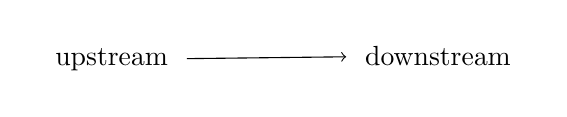
\begin{tikzpicture}
  \matrix (m) [matrix of math nodes, row sep=4.8em, column sep=5.8em, minimum width=2.2em]
  {
\text{ upstream } & \text{ downstream } \\ 
};
  \path[->]
  (m-1-1) edge node [above] {$ $} (m-1-2);
\end{tikzpicture}  \\
 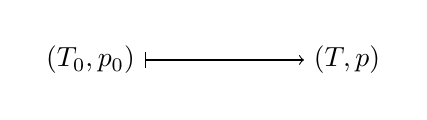
\begin{tikzpicture}
  \matrix (m) [matrix of math nodes, row sep=4.8em, column sep=5.8em, minimum width=2.2em]
  {
(T_0,p_0) & (T,p) \\ 
};
  \path[|->]
  (m-1-1) edge node [auto]  {$$} (m-1-2)
  ;
\end{tikzpicture}   \\
 \frac{T_0}{T} = 1 + \frac{\gamma -1}{2} \mathfrak{M}^2 \\ 
 \frac{p_0}{p} = \left( 1 + \frac{\gamma -1}{2} \mathfrak{M}^2 \right)^{\frac{\gamma}{\gamma -1} }
\end{gathered}
\]

Thus, when one considers heat addition, the thermodynamic process, $\Delta \dot{q}$ occurs on stagnation temperature, and then can be related to the actual, physical fluid flow and its properties, through formulae we've derived: \\
 \begin{tikzpicture}
  \matrix (m) [matrix of math nodes, row sep=4.8em, column sep=5.8em, minimum width=2.2em]
  {
    x_0   \\
    x_1 \\
};
  \path[|->]
  (m-1-1) edge node [auto] {$u$} (m-2-1)
  ;
\end{tikzpicture} 
 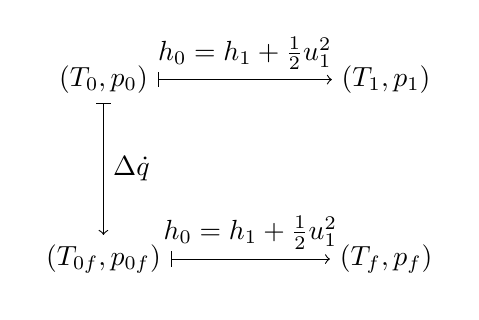
\begin{tikzpicture}
  \matrix (m) [matrix of math nodes, row sep=4.8em, column sep=5.8em, minimum width=2.2em]
  {
    (T_0,p_0) & (T_1,p_1)  \\
    (T_{0f},p_{0f}) & (T_f,p_f) \\ 
};
  \path[|->]
  (m-1-1) edge node [auto] {$h_0 = h_1 + \frac{1}{2}u_1^2$} (m-1-2)
          edge node [auto] {$\Delta \dot{q}$} (m-2-1)
  (m-2-1) edge node [auto] {$h_0 = h_1 + \frac{1}{2}u_1^2$} (m-2-2)
  ;
\end{tikzpicture} 

\begin{lstlisting}
(1.*10**6)/(40.*15.6)
# 1602.5641025641025
\end{lstlisting}
So
\[
\Delta T_0 = 1602.6 \, K
\]
\item[(b)] Now consider the converging section at the inlet to each 1 \, $cm$ diameter channel, that ``accelerates the flow to a relatively low Mach number and produces a flow rate of $40 \, g/s$''.  

Mass continuity (conservation) still holds:
\[
\begin{gathered}
  \dot{m} = \rho A u = \frac{p}{RT} A \mathfrak{M} \sqrt{ \gamma RT } = \frac{p}{\sqrt{RT}} A\mathfrak{M} \sqrt{\gamma } = \frac{p_0 \sqrt{\gamma }}{ \sqrt{RT_0 } } A \mathfrak{M} (1 + \frac{\gamma -1}{2} \mathfrak{M}^2 )^{ \frac{\gamma+1}{-2(\gamma -1) } }
\end{gathered}
\]
where the ``pullback'' to the stagnation properties for each point of the flow, before the converging section and after the converging section, was used:
\[
\begin{aligned}
  & \frac{p_0}{p} = \left( 1 + \frac{\gamma-1}{2} \mathfrak{M}^2 \right)^{\frac{\gamma}{\gamma -1} } \\
  &  \frac{T_0}{T} = 1 + \frac{\gamma-1}{2} \mathfrak{M}^2
\end{aligned}
\]
\begin{lstlisting}
massconsEq = Eq(massflow,p_0*sqrt(gamma/(R*T_0))*A*Mach*(1+(gamma-Rat(1))/Rat(2)*Mach**2)**\
((gamma+1)/(-Rat(2)*(gamma-1))))
massconsProb0503 = massconsEq.subs(massflow,40.*10**(-3)).subs(gamma,1.4).subs(p_0,6.8*10**(6)).\
subs(T_0,673.).subs(A,N(pi)*(10**(-2)/2.)**2).subs(R,k_Boltz.Value/(Decimal(2.0159*10**(-3))/N_Avog.Value))
\end{lstlisting}
where for $R$, $R = \frac{k_B}{M}$ and where for $M$, I used $2.0159 g/\text{mol}$ for \ce{H2}, and Avogadro's number, $N_A = 6.022140857\times 10^{23}$, which is number of particles per mole.  So in this example, $R = 4124.4$ for \ce{H2} as
\begin{lstlisting}
>>> k_Boltz.Value/(Decimal(2.0159*10**(-3))/N_Avog.Value)
Decimal('4124.440627733807619868515695')
\end{lstlisting}

Let's try to use the derived relation, relating the stagnation temperatures before and after (denoted $1$) heat addition:
\[
\frac{T_0}{T_{01}} = \left[ \frac{ 1 + \gamma \mathfrak{M}_1^2 }{1 + \gamma \mathfrak{M}^2}\left( \frac{\mathfrak{M}}{\mathfrak{M}_1}\right)\right]^2\left[\frac{1+\frac{\gamma-1}{2}\mathfrak{M}^2}{1+\frac{\gamma-1}{2}\mathfrak{M_1}^2}\right]
\]
This is implemented in \verb|NozzleTheory.py|:
\begin{lstlisting}
T_01=Symbol('T_01',real=True)
heataddTvsMachEq=Eq(T_0/T_01,((Rat(1)+gamma*Mach_1**2)/(Rat(1)+gamma*Mach**2)*Mach/Mach_1)**2*\
(Rat(1)+(gamma-Rat(1))/Rat(2)*Mach**2)/(1+(gamma-Rat(1))/Rat(2)*Mach_1**2) )

heataddTvsMachProb0503=heataddTvsMachEq.subs(gamma,1.4).subs(T_0,675).subs(T_01,675+(1.*10**6)/\
(40.*15.6)).subs(Mach,MachProb0503)
Mach1Prob0503lamb=lambdify(Mach_1,heataddTvsMachProb0503.rhs-heataddTvsMachProb0503.lhs)
plot(heataddTvsMachProb0503.rhs,(Mach_1,0,10))
Mach1Prob0503=scipy.optimize.newton(Mach1Prob0503lamb,0.1)
\end{lstlisting}
where $\mathfrak{M}$ was obtained for the acceleration by the converging nozzle, $T_0$ is the stagnation temperature that was given, and $T_{01}$ is obtained from part (a).  

Thus,
\[
\mathfrak{M}_1 = 0.2024
\]
The flow through the channel isn't thermally choked as $\mathfrak{M}$ doesn't become $1$ by the heat addition.  
\item[(c)] After exiting the ducts, the converging-diverging nozzle results in a Mach number given by
\[
\frac{A_e}{A^*} = \frac{1}{\mathfrak{M}} \left[ \left( \frac{1 + \frac{\gamma-1}{2} \mathfrak{M}^2 }{ \frac{\gamma+1}{2} } \right)^{\frac{\gamma+1}{\gamma-1} } \right]^{1/2}
\]
and from the Mach number definition and energy equation (Bernoulli invariant), we can get the exhaust velocity
\[
u_e = \mathfrak{M}a = \mathfrak{M}\sqrt{\gamma RT} = \mathfrak{M} \sqrt{ \gamma R \frac{ T_0 }{ 1 + \frac{\gamma-1}{2} \mathfrak{M}^2 } }
\]
\end{enumerate}


\part{Basic Feeling}

\section{Box with a hole rocket; bottled (box) rocket}

Recall Ch. 14: Kinetic Theory, Section ``Kinetic Theory of the Ideal Gas Law'' of Kittel and Kroemer \cite{CKittelHKroemer1980}.

\subsection*{Kinetic Theory of the Ideal Gas Law}

Consider molecule strike unit area of wall. \\
Let $v_z \equiv $ velocity component normal to plane of wall. \\
Suppose molecules, of mass $M$, reflected specularly (mirror-like) from wall,
\[
\Delta p_z = -2M|v_z|
\]
Let $a(v_z)dv_z$, number of molecules per unit volume with $z$-component of velocity between $v_z$ and $v_z + dv_z$.  
\[
\int a(v_z)dv_z = \frac{N}{V} = n
\]
$a(v_z) v_z dv_z$ number of molecules in $(v_z, v_z + dv_z)$  velocity range that strike unit area of wall in (per) unit time
\[
\text{pressure } p = \int_0^{\infty}2M v_za(v_z)v_z dv_z = M\int_{-\infty}^{\infty}v_z^2 a(v_z) dv_z = Mn\langle v_z^2 \rangle
\]
$\frac{1}{2}M\langle v_z^2 \rangle = \frac{1}{2} \tau$ by equipartition of energy (Ch.3)
\[
p = nM \langle v_z^2 \rangle = n\tau = \frac{N\tau}{V}
\]
\subsubsection*{Maxwell Distribution of Velocities}  

cf. Ch.6. distribution function of ideal gas $f(\epsilon_n) = \lambda \exp{ \left( \frac{-\epsilon_n}{\tau} \right)}$

Recall, Ch. 6, Sec. ``Classical Limit'' of Kittel and Kroemer \cite{CKittelHKroemer1980}, \textbf{an ideal gas is defined as a system of free noninteracting particles in the classical regime}.  \\
$f(\epsilon) \equiv $ average occupancy of an orbital at energy $\epsilon$ \\
$\epsilon \equiv $ energy of orbital occupied by 1 particle; not energy of system of $N$ particles \\
Fermi-Dirac and Bose-Einstein distribution $f(\epsilon) = \frac{1}{ \exp{ [ (\epsilon - \mu )/\tau ] } \pm 1 }$ \\
In order for $f(\epsilon) \ll 1$ $\forall \, $ orbitals, $\exp{ [ (\epsilon-\mu)/\tau ] } \gg 1\, \forall \, \epsilon$.  
\[
\Longrightarrow f(\epsilon) \simeq \exp{ [(\mu - \epsilon )/\tau]} = \lambda \exp{ (-\epsilon/\tau)} \quad \, \lambda \equiv \exp{ \left( \frac{ \mu }{\tau} \right) }
\]
$f(\epsilon)$, average occupancy of orbital of energy $\epsilon$, is classical distribution function.  

particle in a box: $\epsilon_n = \frac{1}{2M} \left( \frac{\pi n}{L} \right)^2 $ (for, recall $\frac{1}{2M} \left( \frac{1}{i} \partial \right)^2 \psi = \frac{-1}{2M} \partial^2 \psi = E \psi$)

number of orbitals in range of quantum number $(n,n+dn)$, probability such orbital is occupied

\[
(\frac{1}{2} \pi n^2 dn)f(\epsilon_n) = \frac{1}{2} \pi n^2 \lambda \exp{ (-\epsilon_n/\tau) } dn
\]
\[
\frac{1}{2} Mv^2 = \frac{1}{2M} \left( \frac{ \pi n}{ L } \right)^2 \text{ or } n^2 = \frac{ (ML)^2 }{ \pi^2} v^2 \text{ or } n = \frac{MLv}{\pi}
\]

Consider system of $N$ particles in volume $V$.  

Let $NP(v) dv$ number of atoms with velocity magnitude in range $dv$ at $v$
\[
NP(v) dv = \frac{1}{2} \pi n^2 \lambda \exp{ ( -\epsilon_n /\tau)} \frac{dn}{dv} dv = \frac{1}{2} \pi \lambda \left( \frac{ ML }{ \pi } \right)^3 v^2 \exp{ \left( \frac{ -Mv^2 }{2\tau } \right) }dv
\]
cf. Ch. 6, $\lambda = \frac{n}{n_Q} = \frac{N}{L^3} \left( \frac{ 2\pi \hbar^2 }{ M \tau } \right)^{3/2}$

\[
\frac{1}{2} \pi \frac{N}{L^3} \left( \frac{2\pi }{ M \tau} \right)^{3/2} \left( \frac{ ML }{\pi } \right)^3 = 4\pi N \left( \frac{N}{2\pi \tau} \right)^{3/2}
\]
\begin{equation}
\Longrightarrow P(v) = 4\pi \left( \frac{M}{2\pi \tau } \right)^{3/2} v^2 \exp{ \left( \frac{- Mv^2}{ 2\tau } \right) } 
\end{equation}
$P(v)$ is \textbf{Maxwell velocity distribution}, $P(v)dv$ is probability particle has speed in $dv$ at $v$

\subsubsection*{Experimental verification}

velocity distribution of atoms which exit from slit of oven.  

exit beam weighted in favor of atoms of high velocity at expense of those at low velocity. 

weight factor is velocity component $v\cos{\theta}$ normal to plane of hole. 

\[
\begin{gathered}
  \int (\cos{\theta}) dr rd\varphi r \sin{\theta} d\theta = (\frac{1}{3} (2\pi ) R^3) \int \cos{\theta} \sin{\theta} d\theta = ( \frac{2\pi}{3} R^3) \int \frac{\sin{2\theta} d\theta}{ 2 } = \frac{2\pi R^3}{3} \left. \left( \frac{ - \cos{2\theta} }{4} \right) \right|_0^{\pi/2} = \\
  = \frac{ 2\pi R^3}{3} \left( \frac{1+ 1}{4} \right) = \frac{ 2\pi R^3}{3} \left( \frac{1}{2} \right)
\end{gathered}
\]
Probability atom leaves hole will have velocity in $(v,v+dv)$ : $P_{\text{beam}}(v) dv$

\[
P_{\text{beam}}(v) \propto vP_{\text{Maxwell} } \propto v^3 \exp{ \left( \frac{ -Mv^2}{ 2\tau } \right) }
\]
with, recall $P_{\text{Maxwell}} = 4\pi \left( \frac{ M }{ 2\pi \tau } \right)^{3/2} v^2 \exp{ \left( \frac{-Mv^2}{ 2\tau } \right) }$ 

$P_{\text{beam}}$ distribution of transmission through a hole is Maxwell transmission distribution. 

\begin{equation}\label{Eq:meanvofairbeamouthole}
\begin{gathered}
  \langle v_{\text{out}} \rangle = \int \int_0^{\pi/2} v\cos{\theta} \sin{\theta} d\theta P_{\text{Maxwell}}(v) dv = 4\pi \left( \frac{ M}{ 2\pi \tau} \right)^{3/2} \frac{1}{2} \int_0^{\infty} v^3 \exp{ \left( \frac{-M}{2\tau} v^2 \right) } dv = \\
  = 4\pi \left( \frac{M}{2\pi \tau} \right)^{3/2} \frac{1}{2} \left( \frac{1}{-2\alpha} \right) \left[ 0 - \frac{1}{\alpha} \right] = 4\pi \left( \frac{ M}{2\pi \tau} \right)^{3/2} \frac{1}{4} \left( \frac{4\tau^2}{M^2} \right) = \boxed{ \frac{ 2^{1/2} }{ \pi^{1/2} } \left( \frac{\tau}{M} \right)^{1/2} }
\end{gathered}
\end{equation}
for (doing the integration by hand) 
\[
\begin{aligned}
  & (e^{-\alpha v^2} )' = -2\alpha v e^{-\alpha v^2} \\
  & (v^2 e^{-\alpha v^2} )' = -2\alpha v^3 e^{-\alpha v^2} + 2v e^{-\alpha v^2} \\ 
  & (v^2 e^{-\alpha v^2} + \frac{e^{-\alpha v^2} }{ \alpha } )' = -2\alpha v^3 e^{-\alpha v^2}
\end{aligned}
\]

Armed with this mean velocity $\langle v_{\text{out}} \rangle$ out of a hole of a box, we want the \emph{thrust} that results on a box if we had a box of air, at some pressure, and at some temperature, and then we punch a hole at one end.  

What's happening?  Air that's swirling around the box is then accelerated out of the hole.  There's fluid flow out.  For low enough velocities, use \emph{Bernoulli's equation}, and assume at the starting point of the air's streamline, the velocity is $0$:
\[
\begin{gathered}
  \frac{1}{2} u^2 + \frac{p}{\rho} = \frac{1}{2}u_f^2 + \frac{p_f}{\rho_f} \\
  \Longrightarrow \frac{p}{\rho}  = \frac{1}{2} u_f^2 + \frac{p_f}{\rho_f}
\end{gathered}
\]
$\rho$ is really $\frac{MN}{V}$ and by the ideal gas law (still applies), $pV=N\tau$ and $\frac{p}{\tau} = \frac{N}{V}$ but the point is the gas density didn't change much.  

% https://en.wikibooks.org/wiki/LaTeX/Picture
% cf. http://timmurphy.org/2010/08/20/drawing-pictures-in-latex/
\setlength{\unitlength}{1cm}
\begin{picture}(10, 5)(-1, -1)
\put(0,0){\line(0,4){4}}
\put(0,0){\line(4,0){4}}
\put(0,4){\line(4,0){4}}
\put(4,0){\line(0,1){1.75}}
\put(4,4){\line(0,-1){1.75}}
\end{picture}

Thus,
\[
\begin{gathered}
  \frac{p -p_f}{\rho} = \frac{1}{2} u_f^2
\end{gathered}
\]
The thrust is going to be given by the difference in pressure against the walls, the wall in front of the box opposite to the wall with a hole.  \emph{You don't need the area of the hole.}  This thrust is $(p-p_f)$
\[
\begin{gathered}
  (p-p_f)A = \rho \frac{1}{2} u_f^2 A = \frac{MN}{V} \frac{1}{2}u_f^2 A = \frac{MN}{L} \frac{1}{2}u_f^2
\end{gathered}
\]
Now from Eq. \ref{Eq:meanvofairbeamouthole}, $u_f^2 = \frac{2}{\pi} \frac{\tau}{M}$, and so 
\[
(p-p_f)A = \frac{N\tau}{\pi L} = \frac{pV}{\pi L} = \frac{pL^2}{\pi}
\]
Thus, the thrust on this box is given by 
\[
F_{\text{thrust}} = \frac{N\tau}{\pi L} = \frac{pL^2}{\pi}
\]




\part{Notes and Solutions for \emph{Thermal Physics} by Ralph Baierlein}\cite{RBaierlein1999}

\section{Background}

\subsection{Heating and Temperature}

Heating: keep in mind 3 different types of heating for energy exchange between two systems:

\begin{enumerate}
  \item Heating by conduction - literal contact, molecules jiggle faster from molecules jiggling faster by bouncing off them
  \item Heating by radiation - em waves from hot source strike and excite target
  \item heating by convection - energy transport by flow (perhaps a fluid)
\end{enumerate}

This all relates to \\
$Q$

\subsection{Some dilute gas relationships}

\subsubsection*{Pressure according to kinetic theory} i.e. some kinetic theory

$F \equiv $ force on area $A$ due to molecules \\
$\Delta p \equiv $ momentum transferred to wall per collision \\
$n \equiv$ number of collisions in time $\Delta t$

Thus
\[
F = \frac{ (\Delta p)n }{ \Delta t }
\]

Now $\Delta p = 2 m v_x$ since $\Delta p = mv_x - (-mv_x) = 2mv_x$ (elastic collision with momentum conversation)

$v_x \Delta t A$ is a volume, inside of which gas molecules can be within distance $v_x \Delta t$ toward the wall.  \\
$\frac{N}{V}$ number density of molecules

Assume equal distribution of velocities: Thus $\frac{1}{2}$
\[
 n = (v_x \Delta t A) \frac{1}{2} \frac{N}{V}
\]
\[
P = \frac{F}{A} = \frac{ (2mv_x)(v_x \Delta t A ) \frac{1}{2} \frac{N}{V} }{ A \Delta t} = mv_x^2 \frac{N}{V}
\]

Suppose $\langle v^2 \rangle = \langle v_x^2 \rangle + \langle v_y^2 \rangle + \langle v_z^2 \rangle = 3 \langle v_x^2 \rangle = d \langle v_x^2 \rangle$.  
\[
\Longrightarrow P = \frac{mN}{dV} \langle v^2 \rangle = \frac{2}{d} \frac{1}{2} m \langle v^2 \rangle \frac{N}{V}
\]

\subsubsection*{An empirical gas law}
Now 
\[
P = \frac{N\tau}{V} \quad \, \text{(empirical)}
\]

\[
\Longrightarrow \frac{1}{2} m \langle v^2 \rangle = \frac{d}{2} \tau
\]

\subsection{The First Law of Thermodynamics}

\[
dU = Q - W \text{ or } Q = dU + W 
\]

Consider $W = Q-dU$.  

Consider path in $M$, $\gamma$, $\begin{aligned} & \quad \\
  & \gamma : \mathbb{R} \to M = (U,V) \\
  & \gamma(t) = (U(t), V(t)) \end{aligned}$

$\dot{\gamma} \in \mathfrak{X}(M)$, $\dot{\gamma} = \dot{U} \frac{\partial }{ \partial U} + \dot{V} \frac{ \partial }{ \partial V}$

\[
W(\dot{\gamma}) = pdV(\dot{\gamma}) = p\dot{V} = Q(\dot{\gamma}) - dU(\dot{\gamma}) = Q(\dot{\gamma}) - \dot{U}
\]
Suppose $Q(\dot{\gamma}) = Q(t)dt(\dot{\gamma} \frac{ \partial }{ \partial t} ) = Q(t) \dot{\gamma}$.  
\[
\begin{gathered}
  \int p \dot{V} dt = \int Q(t) \dot{\gamma}dt - \int \dot{U}dt \\ 
  \Longrightarrow p\Delta V = \Delta Q - \Delta U
\end{gathered}
\]
$p\Delta V$ interpreted as work done by gas. $\Delta Q$ is heat transferred to gas system.  $-\Delta U$ is the drop in internal energy of gas system as it does work.  

\subsection{Heat capacity}

\[
Q = Q(\tau,V) = \left( \frac{ \partial Q}{ \partial \tau} \right)_V d\tau +  \left( \frac{ \partial Q}{ \partial V} \right)_{\tau} dV
\]
So define $C_V \equiv \left( \frac{ \partial Q}{ \partial \tau} \right)_V$ or interpret $C_V$ as energy input by heating at constant volume over ensuing change in temperature.  

In this case, $\left( \frac{ \partial U}{ \partial \tau } \right)_V$.  

For the case of a monatomic gas, $U =\frac{d}{2} \tau N$, $\frac{ \partial U}{ \partial \tau} = \frac{d}{2} N$.  
\[
C_V = \frac{d}{2} N
\]
$N \equiv $ number of molecules.  

Now 
\[
\begin{aligned}
  & Q = \Lambda_p dp + C_p d\tau \\ 
  & Q = \Lambda_V dV + C_V d\tau
\end{aligned} \Longrightarrow \begin{aligned}
  & Q \wedge dp = C_p d\tau \wedge dp \\ 
  & Q \wedge dp = \Lambda_V dV \wedge dp + C_V d\tau \wedge dp
\end{aligned}
\]
Now from the thermodynamic identity, $Q = W + dU = pdV + dU$,
\[
Q \wedge dp = p dV \wedge dp + dU \wedge dp
\]
and from (empirical) ideal gas law, $pV = N\tau$ (which defines a hypersurface on $M$),
\[
dp V + p dV = N d\tau \Longrightarrow p dV \wedge dp = N d\tau \wedge dp
\]
so then
\[
Q \wedge dp = N d\tau \wedge dp + dU \wedge dp
\]
In the case of the monatomic gas, $U = \frac{d}{2} \tau N$, and so $dU = \frac{d}{2} N d\tau = C_V d\tau$ and so comparing all the equations above, one recovers
\[
C_p = N + C_V = \frac{2+d}{2} N
\]
EY: 20151019 I'm curious to know how this all generalizes for $C_V$, $C_P$ heat capacities, regardless of the type of molecule we consider.  


\subsubsection*{The adiabatic relation for a classical ideal gas}

Consider the adiabatic expansion (or contraction!) of a classical ideal gas.  \\
This means that $Q=0$; there is no heat exchange to or from the gas system.  

Recall $Q = dU + W$.  \\
If $Q=0$, and supposing $W = pdV$, then $0 = dU + pdV$.  

EY : 20151019 Either by definition, or the thermodynamic identity, $\tau d\sigma = dU + pdV$, then $C_V := \left( \frac{ \partial U}{ \partial \tau} \right)_V$.  My question is this: for manifold of thermodynamic states $M$, $M=(U,V)$, i.e. $U$ is a global coordinate and $V$ is a ``local'' coordinate.  One can make a Legendre transformation such that $M$ is parametrized by $(\tau,V)$, where $\tau$ is the temperature.  In general, one should say that $U=U(\tau,V) \in C^{\infty}(M)$, and so $dU = \frac{ \partial U }{ \partial \tau} d\tau + \frac{ \partial U}{ \partial V} dV$, $dU \in \Omega^1(M)$.    

However, for this adiabatic process, we want
\[
Q = 0 = dU + W = dU + pdV = C_V d\tau + pdV
\]
which implies that $dU = C_V d\tau$.  What happened to the $\frac{ \partial U}{ \partial V} dV$? Is it that in this adiabatic process, the internal energy of the gas system goes to either doing work (expansion) or increases due to work being done on it (contraction), and is characterized completely by a drop or increase in its temperature, respectively?  And so $dU = C_V \tau$, and $pdV$ completely describes what's going on with work done or work done on it?

Nevertheless, using the (empirical) ideal gas law, $pV = N\tau$, 
\[
0 = C_V d\tau + pdV = C_V d\tau + \frac{N\tau}{V} dV
\]
Consider a path $\begin{aligned} & \quad \\
  & \gamma : \mathbb{R} \to M \\ 
  & \gamma(t) = (\tau(t), V(t)) \end{aligned}$ \quad \, in $M$, so that $\dot{\gamma}(t) = \dot{\tau} \frac{ \partial }{ \partial \tau } + \dot{V} \frac{ \partial }{ \partial V} \in \mathfrak{X}(M)$.  

Thus, 
\[
\begin{gathered}
  0 = C_v \dot{\tau} + \frac{N \tau}{V} \dot{V} \text{ so } \frac{ \dot{\tau}}{\tau} + \frac{N}{C_V} \frac{ \dot{V}}{V} \\
  \xrightarrow{ \int dt } \ln{ \frac{ \tau_f}{ \tau_i } } + \frac{N}{C_V} \ln{ \frac{V_f}{ V_i } } = 0 \text{ or } \ln{\tau V^{\frac{N}{C_V}} } = \text{ const. }
\end{gathered}
\]

Now
\[
\frac{N}{C_V} = \frac{C_P - C_V}{ C_V} = \gamma -1 
\]
which is true, assuming the (empirical) ideal gas law, the thermodynamic identity, and, surely, for the case of a monatomic gas.  

Thus
\[
\tau_f V_f^{\gamma-1} = \tau_i V_i^{\gamma -1}
\]

\subsection*{Problems}

\problemhead{4} \emph{Adiabatic compression}. 

A diesel engine doesn't have a spark plug to ignite and explode the fuel.  Instead, the air in the cylinder is compressed so highly that the fuel ignites spontaneously when sprayed into the cylinder.  

\begin{enumerate}
\item[(a)] 
\[
\begin{gathered}
  \frac{ \tau_f V_f^{\gamma -1} }{ \tau_i V_i^{\gamma -1} } = \frac{ P_f V_f^{\gamma }}{ P_i V_i^{\gamma} } = 1 \\
  \tau_f = \left( \frac{V_i}{V_f} \right)^{\gamma -1 }\tau_i
\end{gathered}
\]

Run the Python script \verb|thermo.py| to do the calculations.  Here is (some of) the code from \verb|thermo.py| for doing so (one still needs to import the necessary libraries):

\begin{lstlisting}
roomtemp_K = KCconv.subs(T_C,20).rhs # room temperature in Kelvin                               

Prob0104ans = adia_tV.subs(gamma,1.4).subs(V_f,1).subs(V_i,15).subs(tau_i, roomtemp_K) # answer to Problem 4 of Chapter 1                                                                           

Prob0104ans = N( Prob0104ans.lhs) # 866.016969686253 K                                         
Prob0104ansC = solve( KCconv.subs( T_K, Prob0104ans), T_C )[0] # 592.866969686253 C            
solve( FCconv.subs( T_C, Prob0104ansC ), T_F)[0] # 1099.16054543526 F   
\end{lstlisting}

The final temperature is $866.01 \, K$ or $592.87 \, C$ or $1099.16 \, F$

\item[(b)] Now from the ideal gas law, which is obeyed at all thermodynamic states
\[
\begin{gathered}
  \frac{P_f}{ P_i} = \frac{V_i}{V_f} \frac{ \tau_f}{ \tau_i}
\end{gathered}
\]
and so $\frac{P_f}{P_i} = 44.31$
\end{enumerate}


\section{Phase Equilibrium}

\subsection{Latent heat}

$p,T$ const., liquid $\to $ gas, e.g. $ \begin{aligned} & \quad \\
  & p = 1 \text{ atm } \\
  & T = 373 \, K \end{aligned}$

latent heat of vaporization $L_{\text{vap}}$ (by def.) amount of energy supplied by heating.  \\
$Q = dU + W$ \\
$\epsilon := U/N = $ average (internal) energy per molecule  \\
$v:= V/N = $ volume per molecule 

$L_{\text{vap}} = d\epsilon + p dV$ \\
\phantom{\quad \, } $d\epsilon(\dot{\gamma}) = \epsilon_{\text{vap}} - \epsilon_{\text{liq}}$ \\
\phantom{\quad \, } $dv(\dot{\gamma}) = v_{\text{vap}} - v_{\text{liq}} >0$

if $p$ const., $L_{\text{vap}} = d(\epsilon + pV) = dh$, $h:= H/N = \frac{ U + pV}{N}$

EY : 20151031 A better way to think about it is this: recall that
\[
\begin{aligned}
  & Q = dU + W = dU + pdV = \tau d\sigma \\ 
  & H = U + pV \text{ so } dH = dU + pdV + Vdp = Q + Vdp
\end{aligned}
\]
Consider a path $\gamma \in M$ s.t. $\begin{aligned} & \quad \\
  & d\tau(\dot{\gamma}) = 0 \\
  & dp(\dot{\gamma}) = 0 \end{aligned}$ \quad \, (constant $\tau,p$)

\[
\begin{aligned}
  & Q(\dot{\gamma}) = dH(\dot{\gamma}) - Vdp(\dot{\gamma}) = dH(\dot{\gamma}) - 0 = dH(\dot{\gamma})
  & Q(\dot{\gamma}) = \tau d\sigma(\dot{\gamma}) \\ 
  & \int Q(\dot{\gamma}) = \int \tau d\sigma(\dot{\gamma}) = \tau(\sigma_g - \sigma_l)
\end{aligned}
\]
Thus
\[
\begin{gathered}
  \frac{ \int Q(\dot{\gamma})}{ N} = \tau (s_g - s_l ) = \frac{H_g}{N} - \frac{H_l}{N} \\ 
  L \equiv \tau(s_g - s_l) = \frac{ \int Q(\dot{\gamma})}{ N} = \frac{1}{N} (H_g -H_l)
\end{gathered}
\]

\subsubsection*{Latent heat versus heat capacity}

Take slow, reversible process.  

Now 
\[
\begin{aligned}
  & C_V := \tau \left( \frac{ \partial \sigma }{ \partial \tau} \right)_V \\ 
  & C_P := \tau \left( \frac{ \partial \sigma }{ \partial \tau } \right)_P
\end{aligned}
\]

It's stated in Kittel and Kroemer (1980), pp. 166, Equation (37), Chapter 6: Ideal Gas, Subsection ``Heat capacity'' \cite{CKittelHKroemer1980}, that 
\begin{equation}
  C_P = \tau \left( \frac{ \partial \sigma }{ \partial \tau} \right)_P = \left( \frac{ \partial U }{ \partial \tau} \right)_P + p \left( \frac{ \partial V}{ \partial \tau} \right)_p
\end{equation}

Suppose $\sigma = \sigma(\tau, V)$.  With $\tau d\sigma = dU + W = \tau d\sigma = dU + pdV$, 
\[
\begin{aligned}
  & d\sigma = \frac{ \partial \sigma }{ \partial \tau } d\tau + \frac{ \partial \sigma }{ \partial V} dV = \frac{dU}{ \tau} + \frac{p}{\tau} dV \\ 
  & d\sigma(\dot{\gamma}) = \left( \frac{ \partial \sigma}{ \partial \tau} \right)_V + 0 = \frac{1}{\tau} dU(\dot{\gamma}) = \frac{1}{\tau} \left( \frac{ \partial U}{ \partial \tau} \right)_V
\end{aligned}
\]
Then it's clear that 
\[
\tau \left( \frac{ \partial \sigma }{ \partial \tau } \right)_V = \left( \frac{ \partial U}{ \partial \tau} \right)_V = C_V
\]

Now suppose $\sigma = \sigma(\tau, p)$.  

Consider also the enthalpy,  $H = U + pV$, and so
\[
dH = dU + Vdp + pdV = \tau d\sigma + Vdp
\]
Now for $\sigma = \sigma(\tau,p)$,
\[
\begin{aligned}
  & \sigma = \sigma(\tau,p) \\ 
  & d\sigma = \frac{ \partial \sigma }{ \partial \tau} d\tau + \frac{ \partial \sigma }{ \partial p } dp = \frac{dH}{\tau} - \frac{V}{\tau} dp
\end{aligned} \Longrightarrow d\sigma(\dot{\gamma}) = \left( \frac{ \partial \sigma }{ \partial \tau} \right)_p + 0 = \frac{1}{\tau} \left( \frac{ \partial H}{ \partial \tau} \right)_p - 0 
\]

So 
\[
C_p := \tau \left( \frac{ \partial \sigma }{ \partial \tau } \right)_p = \left( \frac{ \partial H}{ \partial \tau} \right)_p
\]
Now 
\[
\begin{gathered}
  dH(\dot{\gamma}) = dU(\dot{\gamma}) + Vdp(\dot{\gamma} ) + pdV(\dot{\gamma}) = \left( \frac{ \partial U }{ \partial \tau} \right)_p + 0 + p \left( \frac{ \partial V}{ \partial \tau} \right)_p = \left( \frac{ \partial H }{ \partial \tau } \right)_p \text{ so } \\ 
  C_p = \tau \left( \frac{ \partial \sigma }{ \partial \tau} \right)_p = \left( \frac{ \partial U}{ \partial \tau} \right)_p + p\left( \frac{ \partial V}{ \partial \tau} \right)_p 
\end{gathered}
\]

Kittel and Kroemer (1980) \cite{CKittelHKroemer1980} argues that for ideal gas, 
\[
\left( \frac{ \partial U}{ \partial \tau} \right)_p = \left( \frac{ \partial U}{ \partial \tau} \right)_V
\]
since $U = U(\tau)$.  

\subsection{Conditions for coexistence} Sec. 12.3 of Baierlein (1999) \cite{RBaierlein1999}.  

Recall 
\[
G = F + pV = U + pV - \tau \sigma =G(\tau,p,N)
\]

Now 
\[
\begin{gathered}
  G = G(\tau, p, N_{\text{vap}}, N_{\text{liq}} )
\Longrightarrow dG = \frac{ \partial G}{ \partial N_{\text{vap}}} dN_{\text{vap}} + \frac{ \partial G}{ \partial N_{\text{liq}} } dN_{\text{liq}} = \mu_{\text{vap}} 1 + \mu_{\text{liq}} (-1) = 0  \\
\Longrightarrow \mu_{\text{vap}}(\tau,p) = \mu_{\text{liq}}(\tau,p)
\end{gathered}
\]

From Kittel and Kroemer (1980) \cite{CKittelHKroemer1980}, Example : $N$ atoms in a box, Chapter 3: ``Boltzmann Distribution and Helmholtz Free Energy'', 

state of energy $\epsilon_{\alpha}(1) + \epsilon_{\beta}(2) + \dots + \epsilon_{\xi}(N)$, $\alpha, \beta, \dots \xi$ denote orbital indces of atoms in successive boxes.  \\
each entry occurs $N!$ times in $Z_1^N$ (EY: 20151022) $N!$ ways to fill $\alpha, \beta \dots \xi$ orbitals with $N$ distinguishable particles.  Thus,
\[
Z_N = \frac{1}{N!} Z_1^N = \frac{1}{N!} (n_Q V)^N
\]


\part{Notes and Solutions on \emph{Fundamentals of Thermodynamics}, 8th Edition, by Claus Borgnakke, Richard E. Sonntag}
\cite{CBorgnakkeRSonntag2012}

\section{}

\section{Properties of a Pure Substance}

EY : 20151030 Is the word vapor the same as gas?  vapour, gaz, gas, vapore

For coexistence equilibrium, 
\[
\begin{aligned}
  & \mu_g(p_0,\tau_0) = \mu_l(p_0,\tau_0) \text{ and } \\ 
  & \mu_g(p_0 + dp, \tau_0+d\tau) = \mu_l(p_0 + dp, \tau_0+d\tau)
\end{aligned}
\]
and so 
\begin{equation}
  \frac{dp}{d\tau} = \frac{L}{\tau \Delta v}
\end{equation}
where $v\equiv \frac{V}{N}$, the so-called \textbf{vapor pressure equation} or \textbf{Clausius-Clapeyron} equation.  

For (2) approximations, $\Delta v = v_g - v_l \approx v_g = \frac{V_g}{N_g}$ and idealize vapor as ideal gas, $pV = N\tau$ so $\frac{dp}{d\tau} = \frac{L}{\tau^2/p}$.  

Second, if $L$ constant, 
\begin{equation}\label{Eq:CCeq_pvsT}
  p(\tau) = p_0 \exp{ (-L_0/\tau)} \text{ or } \ln{ \left( \frac{p(\tau)}{p_0} \right) } = \frac{-L_0}{\tau}
\end{equation}
cf. Ch. 10 Phase Transformations, pp. 278-284, ``Derivation of the Coexistence Curve, $p$ Versus $\tau$'' of Kittel and Kroemer (1980) \cite{CKittelHKroemer1980}.  

Eq. \ref{Eq:CCeq_pvsT} explains the shape of the coexistence curve between solid and gas (vapor) (sublimation) and liquid and gas (vapor) (vaporization; vaporization curve).  

\textbf{Saturation} is this $p=p(\tau)$ coexistence curve.  


\textbf{Isotherms, Isothermals}

Recall $\begin{aligned} 
  & \quad \\
  & G = F + pV \\
  & F = U-\tau \sigma \end{aligned}$ and so $\begin{aligned}
  & \quad \\
  & dG = dF + Vdp + pdV = dU - \tau d\sigma - \sigma d\tau + pdV + Vdp = -\sigma d\tau + Vdp \\
  & dG = -\sigma d\tau + Vdp \end{aligned}$

So then $\begin{aligned} & \quad \\
  & G = G(\tau, p) \\
  & G= G(\tau, p, N) \end{aligned}$ 

where the latter statement is when we include particle transfer, so that 
\[
dG = -\sigma d\tau + Vdp + \mu dN \text{ for } \mu = \mu(\tau,p)
\]

For the \emph{ideal gas}:

\[
\begin{gathered}
  F(\tau,V) = F= -N\tau \left( \ln{ \left( \frac{n_Q}{n} \right)} + 1 \right) \\ 
  \text{ where }  \begin{aligned}
    & n_Q = \left( \frac{M\tau }{2\pi \hbar^2 } \right)^{3/2} \\ 
    & n \equiv N/V = \frac{p}{\tau} 
  \end{aligned} \\
  G(\tau,p, N) = -N \tau ( \ln{ \left( \frac{n_Q}{n} \right) } + 1 ) + N \tau = - N\tau ( \ln{ \left( \frac{n_Q}{n} \right) } ) = -N\tau \ln{ \left( \left( \frac{M\tau}{2\pi \hbar^2 } \right)^{3/2} \frac{\tau}{p} \right) } \\
  \text{ so then }
\left( \frac{ \partial G}{ \partial N} \right)_{\tau,p} = \mu = -\tau \ln{ \left( \left( \frac{M\tau}{2\pi \hbar^2} \right)^{3/2} \frac{\tau}{p} \right) }
\end{gathered}
\]

For the \emph{Van der Waals gas}
\[
\begin{gathered}
  F(vdW) = -N\tau \left( \ln{ \left( \frac{n_Q (V-Nb)}{N} \right) }  + 1 \right) - \frac{N^2 a }{V} \\ 
  p = -\left( \frac{\partial F}{ \partial V} \right)_{\tau,N} = \frac{N\tau}{V-Nb} - \frac{N^2a}{V^2} \\
  G(\tau,V,N) = \frac{N\tau V}{ V-Nb} - \frac{2N^2 a}{V} - N\tau ( \ln{ \left( \frac{n_Q (V-Nb)}{N} \right) } + 1 )
\end{gathered}
\]

Nevertheless, consider, when considering isotherms, isothermals, 
\[
dG = -\sigma d\tau  + Vdp + \mu dN
\]
Consider a path $\gamma$ on constant $\tau$, constant total number of particles $N$, and so
\[
dG(\dot{\gamma}) = Vdp(\dot{\gamma}) = G_g-G_l = \int_{\gamma} Vdp
\]


\part{Thermodynamics (Revisited)}

\section{Heat Capacity}

From Kittel and Kroemer (1980) \cite{CKittelHKroemer1980}, pp. 165-166, Chapter 6: Ideal Gas, ``Heat Capacity'',
\[
Q = Q(\tau,p) = \Lambda_p dp + C_p d\tau = dU + W = dU + p dV 
\]
Let $c\in \Sigma$ s.t. $dp(\dot{c})=0$ (constant pressure).  And so 
\[
Q(\dot{c}) = 0 + C_p d\tau(\dot{c}) = \tau d\sigma (\dot{c}) = dU(\dot{c}) + pdV(\dot{c})
\]
for $c=(\tau,0)$, $\dot{c} = \frac{\partial }{ \partial \tau} \in T\Sigma$.  

\[
\Longrightarrow C_p = \tau \left( \frac{ \partial \sigma }{ \partial \tau} \right)_p = \left( \frac{ \partial U}{ \partial \tau} \right)_p + p \left( \frac{ \partial V}{ \partial \tau} \right)_p
\]
for heat capacity at constant pressure is larger than $C_V$ because additional heat must be added to perform the work needed to expand volume of gas against constant pressure.  

Now recall for enthalpy 
\[
\begin{aligned}
  & H = U+ pV \\ 
  & H = H(\sigma, p)
\end{aligned}
\]
Then
\[
dH = dU+ pdV + Vdp = Q + Vdp 
\]
Thus, for $c\in \Sigma$, $dp(\dot{c})=0$ (constant pressure).  Hence
\[
dH(\dot{c}) = \left( \frac{ \partial H}{ \partial \tau} \right)_p = Q(\dot{c})  +  0 = C_p
\]
Hence, 
\[
C_p = \left( \frac{ \partial H}{ \partial \tau } \right)_p = \left( \frac{ \partial Q}{ \partial \tau} \right)_p
\]



\section{Phase Equilibrium}


\begin{description}
\item Phase Equilibrium
\item Phase Diagram
\item (Phase) Coexistence Curve 
\item Antoine Equation (parameters)
\end{description}


For coexistence equilibrium, $\mu_g(p_0,\tau_0) = \mu_l(p_0,\tau_0)$ and $\mu_g(p_0 + dp, \tau_0 + d\tau) = \mu_l(p_0 + dp, \tau_0+d\tau)$, and so $\frac{dp}{d\tau} = \frac{L}{ \tau \Delta v}$ with $v \equiv \frac{V}{N}$.  

Make the approximation that $\Delta v \equiv v_g - v_l \approx v_g = \frac{V_g}{N_g}$ and idealize vapor as ideal gas, $pV = N\tau$, so $\frac{dp}{d\tau} = \frac{L}{\tau^2/p}$.  

If $L$ constant, 
\begin{equation}
p(\tau) = p_0 \exp{ (-L_0 /\tau)} \text{ or } \ln{ \left( \frac{p(\tau)}{p_0} \right) } = \frac{-L_0}{\tau}
\end{equation}

Consider the Antoine Equation Parameters given in the NIST (National Institute of Standards and Technology) Chemistry WebBook \footnote{\href{http://webbook.nist.gov/cgi/cbook.cgi?ID=C7782447&Mask=4\#Thermo-Phase}{Phase change data for Oxygen}}

\begin{equation}
  \log_{10}(P) = A- (B/(T+C))
\end{equation}

Then
\[
\begin{gathered}
  P = 10^{ A = \frac{B}{T+C}} = 10^A 10^{-\frac{B}{T+C}} = 10^A \exp{ \left( \frac{-B}{T+C} \ln{10} \right) }
\end{gathered}
\]
Now $\frac{D}{T+C} = \frac{D}{T} - \frac{DC}{T(T+C)}$, and so
\[
P = 10^A \exp{ \left( \frac{ (B\ln{10} )C }{T(T+C)} \right) }\exp{ \left( \frac{-B\ln{10} }{ T} \right) }
\]
Consider how much the pressure is changed due to this $C$ parameter.  Consider $P_0$, $P_1$, defined as such:
\[
\begin{gathered}
  \begin{aligned}
    & P_0 = 10^A  \exp{ \left( \frac{-B\ln{10} }{ T} \right) }
    & P_1 = 10^A \exp{ \left( \frac{ (B\ln{10} )C }{T(T+C)} \right) }\exp{ \left( \frac{-B\ln{10} }{ T} \right) }
  \end{aligned} \Longrightarrow \frac{P_0}{P_1} = \exp{ \left( \frac{ (B\ln{10} )C }{ T(T+C) } \right)}
\end{gathered}
\]
So a deviation can be estimated from $1 - \frac{P_0}{P_1}$.  

Open up \verb|thermochem.py|.  The \emph{saturation curve} or \emph{coexistence curve} for, for example, oxygen, from liquid to gas, can be reproduced.  One needs to input in the Antoine parameters from the NIST website \footnote{\url{http://webbook.nist.gov/cgi/cbook.cgi?ID=C7782447&Mask=4\#Thermo-Phase}}

\begin{lstlisting}
>>> O2coec = CoexistCurve(3.85845, 325.675, -5.667 )                                            
>>> plot( O2coec.curveSI.rhs, (T,54.36,100.16) )   

>>> N(O2coec.curveSI.rhs.subs(T,60.))
731.804072053687
>>> N(O2coec.curveSI.rhs.subs(T,70.))
6253.42680398774
>>> N(O2coec.curveSI.rhs.subs(T,75.))
14494.1195824433
\end{lstlisting}

  \quad \quad \quad







%\begin{figure}[b]
%  \centering
%  \includegraphics[width=\columnwidth]{../eps/Nielsen2011RBB_qualitative_report_topicsentiment}
%  \caption{Web service screenshot with text from Wikipedia
%    article ``Lundbeck''.}
%  \label{fig:topicsentiment}
%\end{figure}






\end{multicols*}

\begin{thebibliography}{9}

\bibitem{GSuttonOBiblarz2001}
George P. Sutton, Oscar Biblarz. \textbf{Rocket Propulsion Elements}, 7th Edition. Wiley, 2001.  
 

\bibitem{RBaierlein1999}
Ralph Baierlein. \textbf{Thermal Physics} Cambridge University Press (July 28, 1999), ISBN-13: 978-0521658386

\bibitem{CKittelHKroemer1980}
Charles Kittel, Herbert Kroemer, \textbf{Thermal Physics}, W. H. Freeman; Second Edition edition, 1980. 
ISBN-13: 978-0716710882

\bibitem{BSchutz1980}
Bernard F. Schutz, \textbf{Geometrical Methods of Mathematical Physics}, Cambridge University Press, 1980.
ISBN-13: 978-0521298872

\bibitem{CBorgnakkeRSonntag2012}
Claus Borgnakke, Richard E. Sonntag.  \textbf{Fundamentals of Thermodynamics}, 8th Edition, Wiley, (December 26, 2012). 
ISBN-13: 978-1118131992  

\end{thebibliography}
There's an 8th edition of Biblarz and Sutton \cite{GSuttonOBiblarz2001} for 2010 that I would like to have.  If you find any of this material useful or if you'd like to help, email me or visit my Open/Tilt page \url{ernestyalumni.tilt.com} and donate to the crowdfunding campaign or click on the PayPal donate button.  






\clearpage
\onecolumn

\section{Code listings}

\definecolor{darkgreen}{rgb}{0, 0.4, 0}
\lstset{language=Python,
  numbers=left,
  frame=bottomline,
  basicstyle=\scriptsize,
  identifierstyle=\color{blue},
  keywordstyle=\bfseries,
  commentstyle=\color{darkgreen},
  stringstyle=\color{red},
  literate={Ö}{{\"O}}1 {é}{{\'e}}1 {Å}{{\AA}}1,
}
\lstlistoflistings


%\label{listing:brede_str_nmf}\lstinputlisting{../../matlab/brede/python/brede_str_nmf}


\newpage
\section{Automatic generation of documentation}

Demontration using epydoc:
\begin{verbatim}
epydoc --pdf -o /home/fnielsen/tmp/epydoc/ --name RBBase wikipedia/api.py
\end{verbatim}
This example does not use \verb!brede_str_nmf! but another more
well-documented module called {\tt api.py} that are used to download
material from Wikipedia. 

%\includepdf[pages={-}]{/home/fnielsen/tmp/epydoc/api.pdf}

\end{document}
